% =====================================================================================
% The Monetary-Financial-Fiscal Macromodel (MFFM): A Global Projection and Scenario Tool
% Adrian - Farkas - Linde
%
% STYLE CONTRACT (binding, per author guidance):
%   - Plain words before equations. Every term defined at first use. No undefined jargon.
%   - Every experiment answers: what do we do, how do we do it, what do we find.
%   - Every quoted number is a macro from constants.tex (script-generated; never hand-typed).
%   - Technical material lives in the appendices, not the main text.
% BUILD: pdflatex mffm_platform_paper && bibtex mffm_platform_paper && pdflatex x2
% =====================================================================================
\documentclass[11pt]{article}

\usepackage[a4paper,margin=1.1in]{geometry}
\usepackage{amsmath}
\usepackage{amssymb}
\usepackage{booktabs}
\usepackage[round,authoryear]{natbib}
\usepackage{graphicx}
\usepackage{longtable}
\usepackage{xcolor}
\usepackage{pgfplots}
\pgfplotsset{compat=1.17}
\usepgfplotslibrary{groupplots}
\usepackage{hyperref}
\hypersetup{colorlinks=true,linkcolor=black,citecolor=blue,urlcolor=blue}

% ---- figure panel styles (all §3 figures share these) ----
\definecolor{scenblue}{RGB}{31,79,141}
\definecolor{naivered}{RGB}{196,69,28}
\definecolor{jointgreen}{RGB}{20,120,80}
\pgfplotsset{
  paperpanel/.style={width=0.36\textwidth, height=0.27\textwidth,
    xmin=1, xmax=20, xlabel={quarters}, xlabel near ticks,
    tick label style={font=\scriptsize}, label style={font=\scriptsize},
    title style={font=\small}, axis line style={gray!70}, tick style={gray!70}},
  zeroline/.style={gray!55, thin, forget plot},
  trueline/.style={scenblue, thick},
  naiveline/.style={naivered, thick, dashed},
  globline/.style={scenblue, thick},
  usoline/.style={naivered, thick, dotted},
  jointline/.style={jointgreen, thick, dashed},
  cfline/.style={jointgreen, thick, dashed},
}

% constants.tex — every number quoted in the paper lives here, ONE definition per fact.
% HAND-SEEDED for the skeleton from the shipped V3 artifacts (branch effi-even-seasonal-dummies,
% deployed 2026-07-18, release 3.0.0). Step 3 of the plan replaces this file with a
% SCRIPT-GENERATED version (docs/paper/figs/make_constants.mjs) so no number is hand-typed.
% Sources are noted per line — update ONLY by regeneration.

% --- coverage (source: app/public/data/coverage_manifest.json, weights_24bloc.json blocs) ---
\newcommand{\NBlocs}{38}          % coupled GVAR blocs (euro area = one bloc)
\newcommand{\NMembers}{17}        % euro-area member satellite models
\newcommand{\NModels}{55}         % 38 + 17 country models served by the tool
\newcommand{\NUSVars}{40}         % US bloc variables (spec.json n)
\newcommand{\NLags}{3}            % VAR lag order p
\newcommand{\HorizonQ}{20}        % forecast horizon, quarters

% --- dating (source: app/src/lib/dates.ts, coverage_manifest.json) ---
\newcommand{\LastObsQ}{2026Q1}    % last historical quarter (observed + model-completed)
\newcommand{\NowcastQ}{2026Q2}    % first forecast quarter (the nowcast)

% --- solve (GENERATED: rho_margin.mjs reads the SHIPPED coupling artifact — regenerate, never hand-edit) ---
% GENERATED by app/scripts/paper_figs/rho_margin.mjs from the SHIPPED coupling artifact — do not edit by hand.
\newcommand{\RhoM}{0.97340}       % spectral radius of the coupling map M (power iteration, shipped artifact)
\newcommand{\RhoMargin}{2.66}     % invertibility margin 1-rho(M), percentage points
\newcommand{\RhoBreakPct}{2.73}   % uniform coupling strengthening that pushes rho(M) to 1, percent
\newcommand{\WorldAmpBound}{38}    % worst-case geometric amplification bound 1/(1-rho(M))
\newcommand{\CouplingDim}{2180}      % stacked one-quarter system dimension (rows of M)


% --- Bayesian-GVAR comparison (GENERATED: ccfh_headtohead.mjs parses the ccfh_replication RESULTS files) ---
% GENERATED by app/scripts/paper_figs/ccfh_headtohead.mjs from the ccfh_replication RESULTS files — do not edit by hand.
\newcommand{\GbvarYHOne}{0.87}    % G-BVAR relRMSE vs AR5, output, h=1 (v5 run — same run as the CCFH appendix)
\newcommand{\GbvarYHFour}{0.78}   % G-BVAR relRMSE vs AR5, output, h=4 (v5 run)
\newcommand{\CcfhSzStirHFour}{2.58}  % CCFH reproduction: S&Z/AR relRMSE, short rate, h=4 (their code+data)
\newcommand{\CcfhDiffuseStirHFour}{6.95} % CCFH reproduction: diffuse/AR relRMSE, short rate, h=4
\newcommand{\CcfhSzYHOne}{0.95}       % CCFH reproduction: S&Z/AR relRMSE, output, h=1

% --- CCFH-design appendix (GENERATED: ccfh_matrix.mjs — full matrix + regional cut) ---
% GENERATED by app/scripts/paper_figs/ccfh_matrix.mjs — do not edit by hand.
\newcommand{\CmGbvarYHOne}{0.87}
\newcommand{\CmGbvarYHFive}{0.75}
\newcommand{\CmGbvarYHNine}{0.64}
\newcommand{\CmGbvarRHNine}{0.72}
\newcommand{\CmGbvarRHOne}{0.95}
\newcommand{\CmNostarsYHNine}{0.62}
\newcommand{\CmNostarsYHOne}{0.90}
\newcommand{\CmStarsNostarsGap}{0.08}   % max |stars - nostars| over vars x h
\newcommand{\CmAnchYHNine}{0.62}
\newcommand{\CmAnchRHNine}{0.77}
\newcommand{\CmToolboxYHOne}{0.96}
\newcommand{\CmToolboxYHFive}{1.85}
\newcommand{\CmSsvsYHOne}{1.85}
\newcommand{\CmMnYHNine}{0.87}
\newcommand{\CmMnRHOne}{10.50}
\newcommand{\CmRwYHNine}{0.93}
\newcommand{\CmRwRHFive}{0.84}
\newcommand{\CmGbvarYLpsHOne}{5.1}
\newcommand{\CmGbvarYLpsHNine}{7.8}
\newcommand{\CmRegEuYMed}{0.84}
\newcommand{\CmRegEuYIqr}{0.12}
\newcommand{\CmRegAsiaYMed}{0.80}
\newcommand{\CmRegAsiaYIqr}{0.04}
\newcommand{\CmRegSsvsEuYIqr}{1.03}
\newcommand{\CmRegClY}{1.00}
\newcommand{\CmAnchRHOne}{0.99}
\newcommand{\CmAnchRHFive}{0.87}
\newcommand{\CmAnchRMeanHNine}{0.75}
\newcommand{\CmGbvarRMeanHNine}{0.85}
\newcommand{\CmAnchLrHNine}{1.06}
\newcommand{\CmGbvarLrHNine}{0.85}
\newcommand{\CmAnchRLpsHNine}{5.2}
\newcommand{\CmGbvarRLpsHNine}{5.0}
\newcommand{\CmGbvarRHFive}{0.85}
\newcommand{\CmGbvarDpHOne}{1.02}
\newcommand{\CmAnchDpHFive}{1.18}
\newcommand{\CmGbvarDpHFive}{1.00}
\newcommand{\CmRwLrHNine}{0.72}
\newcommand{\CmRwLrHOne}{0.98}
\newcommand{\CmRwEpHNine}{0.73}
\newcommand{\CmGbvarEpHNine}{0.79}
\newcommand{\CmRegSsvsAsiaYIqr}{0.73}
\newcommand{\CmRegMnAsiaYIqr}{0.83}
\newcommand{\CmAnchMeanRHOne}{2.03}
\newcommand{\CmAnchMeanRHNine}{2.10}

% --- own-panel pilot (GENERATED: ourpanel_matrix.mjs parses the eval harness tables) ---
% GENERATED by app/scripts/paper_figs/ourpanel_matrix.mjs — do not edit by hand.
\newcommand{\OpGbvarGHOne}{1.34}
\newcommand{\OpGbvarGHNine}{1.00}
\newcommand{\OpGbvarRHNine}{1.33}
\newcommand{\OpSbvarGHOne}{1.32}
\newcommand{\OpSbvarIHOne}{0.86}
\newcommand{\OpArOneGHOne}{1.10}
\newcommand{\OpAnchIHNine}{1.08}
\newcommand{\OpGbvarIHNine}{1.08}
\newcommand{\OpAnchRHNine}{1.25}
\newcommand{\OpSbvarAnchRHNine}{0.99}
\newcommand{\OpSbvarRHNine}{1.04}
\newcommand{\OpNCells}{24}
\newcommand{\OpArFiveIHNine}{0.52}
\newcommand{\OpArFiveGHNine}{0.85}
\newcommand{\OpCtryIHNine}{0.73}
\newcommand{\OpGbvarIHOne}{0.84}
\newcommand{\OpGbvarIHFive}{0.81}
\newcommand{\OpRwDriftGHOne}{0.93}
\newcommand{\OpAnchRHOne}{1.30}
\newcommand{\OpGbvarRHOne}{0.97}


% --- model structure (source: US spec.json blocks; spec seasonalRows count over app/public/data/bvar) ---
\newcommand{\NGlobals}{four}      % global commons: GLB_OIL, GLB_USLR, GLB_USBAA, GLB_USEQ
\newcommand{\NSeasonal}{18}       % coupled blocs with seasonalRows = 3 (count of spec.json)
\newcommand{\NEvenEffi}{eight}    % evened-interest fiscal blocs (CL CO CR ID IL MX TR ZA)
\newcommand{\NFiscal}{25}         % coupled blocs carrying the 4-variable fiscal block (verified count of spec.json block:'fiscal')

% --- US bloc (source: coverage_manifest estimationSample; weights_24bloc.json US row) ---
\newcommand{\USSampleStart}{1998Q3}
\newcommand{\USSampleEnd}{2025Q4}
\newcommand{\USSampleT}{110}      % estimation quarters
\newcommand{\WUSEA}{0.17}         % US weight on the euro area (rounded, 0.1701)
\newcommand{\WUSMX}{0.16}         % Mexico (0.1625)
\newcommand{\WUSCA}{0.16}         % Canada (0.1623)
\newcommand{\WUSCN}{0.14}         % China (0.1402)

% GENERATED by app/scripts/paper_figs/us_spread_cf.mjs — do not edit by hand.
\newcommand{\NaiveLrImpactBp}{69}    % 10y response, naive pin, impact quarter (bp)
\newcommand{\NaivePolPeakBp}{45}  % policy-rate peak response, naive (bp)
\newcommand{\NaiveLrPeakBp}{69}   % 10y peak response, naive (bp)
\newcommand{\TrueGdpTroughPct}{1.02} % GDP level trough, true spread (% below baseline)
\newcommand{\TrueGdpTroughQ}{4}          % trough quarter (1-based from the nowcast)
\newcommand{\TrueGdpGrowthMinPp}{1.79} % worst q/q-ann growth deviation below baseline (pp, magnitude)
\newcommand{\CFEasingBp}{283}              % unanticipated SW07 easing at q0 (bp), trough-offset sized
\newcommand{\CFResidualPct}{0.00} % GDP dev left at the trough under the CF (%)
\newcommand{\DebtGapHPp}{1.9}   % debt/GDP gap vs baseline at the 5y horizon (pp of GDP)

% GENERATED by app/scripts/paper_figs/global_spread.mjs — do not edit by hand.
\newcommand{\USGdpTroughGlobPp}{2.34} % US growth trough, global solve (pp)
\newcommand{\EAGdpTroughPp}{2.15}   % EA growth trough, US shock, global solve (pp)
\newcommand{\JPGdpTroughPp}{3.48}   % JP growth trough, US shock, global solve (pp)
\newcommand{\WorldTroughUsoPp}{0.54}  % world growth trough, US-only leg (pp)
\newcommand{\WorldTroughGlobPp}{1.95} % world growth trough, global solve (pp)
\newcommand{\WorldTroughJointPp}{2.33}% world growth trough, joint US+EA+JP (pp)
\newcommand{\WorldAmp}{8.7}     % world cumulative effect, global / US-only
\newcommand{\WorldTroughRatio}{3.6} % world TROUGH ratio, global / US-only (the "times as much" the text quotes)
\newcommand{\GlobalSweeps}{1}                        % Gauss-Seidel sweeps to converge

% GENERATED by app/scripts/paper_figs/nfa_pilot.mjs — do not edit by hand.
\newcommand{\ExtUsTbAnchor}{-3.21}    % US trade balance at the nowcast (% of GDP)
\newcommand{\ExtUsCaAnchor}{-3.73}    % US current account PUBLISHED anchor (% of GDP — the sourced caAnchor the text calls "its published value"; the model's nowcast CA = this + one quarter of trade delta)
\newcommand{\ExtUsNfaSeed}{-66.8}        % US net IIP seed nfa0 (% of GDP, sourced FRED IIPUSNETIQ/GDP)
\newcommand{\ExtUsNfaH}{-49.7}       % US NFA/GDP at the 5y horizon, baseline (%)
\newcommand{\ExtEaCaAnchor}{2.8}    % EA current account PUBLISHED anchor (% of GDP, Eurostat)
\newcommand{\ExtCnCaAnchor}{1.89}    % CN current account PUBLISHED anchor (% of GDP, IMF WEO)
\newcommand{\ExtScenCaPeakPp}{0.27}          % peak scenario CA improvement vs baseline (pp of GDP, magnitude)
\newcommand{\ExtScenNfaDevH}{0.25}         % scenario NFA/GDP deviation magnitude at 5y (pp of GDP)


\newcommand{\code}[1]{\texttt{\small #1}}
\newcommand{\todo}[1]{\textcolor{red!70!black}{\small [TODO: #1]}}

\title{\textbf{The Monetary--Financial--Fiscal Macromodel (MFFM):\\
A Global Projection and Scenario Tool}}
\author{Tobias Adrian \and M\'aty\'as Farkas \and Jesper Lind\'e\thanks{%
International Monetary Fund. The views expressed here are those of the authors and do not
necessarily represent the views of the IMF, its Executive Board, or IMF management. We thank
seminar participants at the MCM Financial-oversight-of-the-System meeting for comments.}}
\date{July 2026 --- first draft}

\begin{document}
\maketitle

\begin{abstract}
\noindent Policy questions cross borders, but the tools for answering them mostly do not:
institutions either operate world models that require specialist teams, or stitch
single-country analyses together by hand. This paper documents the MFFM, a platform built to
close that gap. It produces internally consistent projections and scenarios for \NModels{}
economies in a web browser, fast enough to revise them live in a meeting, and everything it
shows comes from one estimated model: a Bayesian vector autoregression for each economy,
linked to its partners through three trade-weighted foreign variables and four global
financial prices, estimated jointly across missing data, and solved as a single linear fixed
point. One example carries the paper from a first click to a policy conclusion. Pinning a 100
basis point rise in the US corporate bond yield does not produce a spread shock, because in
the data corporate yields rarely rise alone; the model raises government yields and the
policy rate with it. Holding the ten-year yield fixed on impact isolates the credit shock;
the global solve then carries it to every economy, deepening the world output loss to about
\WorldTroughRatio{} times what a US-only analysis would show, and a Smets--Wouters counterfactual prices the monetary easing
that would undo the damage. \\[6pt]
\textbf{Keywords:} scenario analysis, conditional forecasting, GVAR, Bayesian VAR, policy
counterfactuals. \quad \textbf{JEL:} C32, C53, E37, E47.
\end{abstract}

% =====================================================================================
\section{Introduction}\label{sec:intro}
% =====================================================================================

When markets move, or a policy changes, or a shock hits somewhere in the world, policymakers
need an answer within days: what does this mean for growth, inflation, and interest rates, at
home and abroad? A useful answer is quantitative, carries its uncertainty with it, and is
consistent --- the view taken for the United States and the view taken for the euro area
cannot rest on contradictory assumptions about the same world. Any central bank produces such
answers for its own economy as a matter of routine. Producing them for many economies at once
is the hard part, and the hard part is what this paper is about.

Scenario analysis is how policy institutions now confront this kind of question. Stress
tests are built on scenarios \citep{AdrianMorsinkSchumacher2020}; growth-at-risk made the
conditional distribution of outcomes, rather than the point forecast, a standard object of
surveillance \citep{AdrianBoyarchenkoGiannone2019}; and the research frontier treats
scenarios themselves as statistical objects, to be checked for concordance with a reference
forecast, weighted by plausibility, and synthesized into a single view of macroeconomic risk
\citep{AdrianGiannoneLucianiWest2025}. Behind all of this stands one requirement. A scenario
is a conditional statement about a joint distribution, and it is only as good as its
conditioning: coherent across variables, so the narrative does not contradict the model, and
coherent across countries, so one desk's downside is not another desk's baseline. Producing
such scenarios --- many of them, quickly, for many economies --- is the unglamorous step on
which the whole edifice rests.

That production step belongs today to specialists, organized in what the profession calls a
suite of models. Central banks and international institutions maintain structural DSGE
models for policy experiments, semi-structural workhorses for the projection process, and
empirical models for forecasting, each run by its own team; the Eurosystem's own review
documents the practice \citep{DarracqPariesEtAl2021}, and the estimated open-economy models
that central banks operate \citep{AdolfsonLaseenLindeVillani2007}, the IMF's Global
Macrofinancial Model \citep{Vitek2018}, and the quantitative model of the Integrated Policy
Framework \citep{AdrianErcegLindeZabczykZhou2020} are all of this kind: powerful, and
staffed. The nearest relative of our platform is the ECB's multi-country model, which
extends the ECB-BASE semi-structural framework to the five largest euro-area countries and
anchors the staff projections \citep{AngeliniBokanChristoffelCiccarelliZimic2019,
AngeliniBokanCiccarelliLalikZimic2025}; we return to it below, because its documentation
sets the standard for papers of this genre. What none of these arrangements solves is
reach. The distance between what a specialist team can supply and what every country desk
needs is well documented from inside the profession \citep{LindeSmetsWouters2016}, so most
desks improvise: single-economy models and judgment, reconciled across borders by
iteration, with one desk's output becoming another's assumption and the aggregation living
in spreadsheets. The result is slow, hard to reproduce, and only as consistent as the last
round. Between the spreadsheet and the specialist model sits the gap this paper addresses:
scenario production that any economist can do, for any economy, with cross-border
spillovers that are consistent by construction.

The MFFM --- the Monetary--Financial--Fiscal Macromodel --- fills that gap by making every
desk a producer. It runs in a web browser, with nothing to install and no code to write, and
opens on a baseline forecast for each of \NModels{} economies, estimated from the latest
published data and covering growth, inflation, interest rates and financial prices, with a
full fiscal block for most economies and uncertainty bands throughout. The \NBlocs{} main
blocs are linked to one another, the euro area entering as one bloc whose outcome its
\NMembers{} members inherit. A scenario is built by \emph{conditioning}: click a variable,
drag its future path or import an outside forecast, and the model recomputes the most likely
path of everything else, in every linked economy. Because the full cross-country solve takes
about a second, a desk economist can build and revise scenarios in the meeting rather than
commission them from a modeling team. In the language of the synthesis literature, the tool
mass-produces the ingredients that scenario synthesis consumes: a reference forecast and
coherent conditional scenarios, for every economy at once, ready to be weighed and
combined.

One estimated model sits behind the screen. Each economy is a Bayesian vector autoregression;
three trade-weighted foreign variables --- partner demand, partner inflation, the partner
short rate --- and four global financial prices tie the economies together, a Bayesian global
VAR in the tradition of \citet{CrespoFeldkircherHuber2016}. Sparse linkage of
this kind is what makes a global model estimable at all, an insight the tool inherits from the
global VAR literature. Two obstacles remain, and the design is built around them. The data are
ragged --- samples of different lengths, publication lags, a pandemic --- so the model treats
missing values as quantities to be estimated, not as reasons to discard data. And interaction
demands speed, which the model delivers by algebra: once estimated, any scenario is a linear
problem, so the world solution is computed once, shipped with the tool, and reused for every
scenario a user tries.

One worked example carries the paper from a first click to a policy conclusion. Ask for a 100
basis point rise in the US corporate bond yield and the model surprises you: government yields
and the policy rate rise too, because in the data corporate yields rarely rise alone. The
surprise teaches the central craft of conditional forecasting --- a scenario is defined as
much by what you hold still as by what you move. One more pin, the ten-year Treasury yield
held at baseline on impact, turns the same rise into a true credit shock: output falls, policy
eases, debt accumulates. The global solve then carries the shock abroad, and a structural
counterfactual --- an unanticipated easing in the model of \citet{SmetsWouters2007}, laid on
top of the scenario --- prices the policy response that would undo the output loss. The parts
of the machine are borrowed, and Section~\ref{sec:method} gives the credits while writing the
model down next to the classical global VAR it descends from; the contribution is the
integration --- one estimable global model, current with the data, solved instantly, usable by
any economist. Section~\ref{sec:example} is the example. Section~\ref{sec:conclusion}
concludes, and the appendices hold the algebra, the testing record, and the commands that
reproduce every figure.

% =====================================================================================
\section{Methodology}\label{sec:method}
% =====================================================================================

% =====================================================================================
% §2 METHODOLOGY — the full econometric treatment (classical GVAR and MFFM in parallel).
% Every constant here is verified against the code: cgl_bvarV5.m (hyperpriors, MH bounds),
% export_bvar_gvar24_loop.m (MAXIT/TOL/draws/WN columns/star construction), the shipped
% coupling artifact (dim, rho). Do not edit numbers by hand.
% =====================================================================================

Two models organize this section, and they are meant to be read against each other. The
classical GVAR comes first, in the form the literature developed it, because the MFFM keeps
its skeleton and the comparison is sharpest with both on the page. The MFFM follows: what a
bloc is, how its foreign variables are built, how the system is estimated and then solved.
The section closes with the question any design must answer --- what this way of working
buys, and what it costs --- and with the US bloc, which runs through everything as the
concrete example. Readers who want the tour first can jump to Section~\ref{sec:example} and
return.

\subsection{The classical GVAR}\label{sec:classical}

The global VAR grew out of a practical need: to extend a national model with the foreign
variables that national outcomes depend on, without attempting an intractable world system.
Proposed by \citet{PesaranSchuermannWeiner2004} and developed fully in
\citet{DeesDiMauroPesaranSmith2007}, it models each economy as a VARX$^{*}$, a VAR augmented
with weakly exogenous foreign variables, and ties the country models into one global system
through trade weights; \citet{ChudikPesaran2016} survey the approach and
\citet{diMauroPesaran2013} collect its applications.

Formally, country $i=1,\dots,N$ is described by a VARX$^{*}(p_i,q_i)$ model,
\begin{equation}\label{eq:varx}
  y_{it} \;=\; a_{i0} \;+\; \sum_{s=1}^{p_i} \Phi_{is}\, y_{i,t-s}
  \;+\; \sum_{s=0}^{q_i} \Lambda_{is}\, y^{*}_{i,t-s}
  \;+\; \sum_{s=0}^{q_i} \Upsilon_{is}\, d_{t-s} \;+\; u_{it},
\end{equation}
where $y_{it}$ is the $k_i\times1$ vector of domestic variables, $y^{*}_{it}$ the
country-specific foreign variables, $d_t$ a small set of global variables (the oil price is
the canonical member), and $u_{it}$ the reduced-form innovation. The foreign variables are
trade-weighted cross sections of the partners' variables,
\begin{equation}\label{eq:starsclassical}
  y^{*}_{it} \;=\; \sum_{j=1}^{N} w_{ij}\, y_{jt}, \qquad w_{ii}=0,
\end{equation}
with fixed weights $w_{ij}$, usually bilateral trade shares.\footnote{The weighting scheme
matters less than one might expect; see \citet[p.~169]{diMauroPesaran2013}.}

Two assumptions make this system estimable country by country. The first is \emph{weak
exogeneity} of $y^{*}_{it}$ and $d_t$ with respect to the parameters of bloc
$i$:\footnote{Foreign variables may affect the domestic economy contemporaneously, but they
are not affected by domestic disequilibria --- the lagged domestic error-correction terms do
not enter the marginal model of the foreign variables
\citep[pp.~56--57]{GarrattLeePesaranShin2012}. Careful applications test this restriction
bloc by bloc rather than assume it.} each economy takes the world as given. That is
plausible for a small open economy and fails, by construction, for the largest one, so the
United States is treated asymmetrically: it is the source of the global variables $d_t$,
and its own foreign-variable set is restricted. The second assumption is a common
estimation window. The blocs are estimated on a shared balanced sample, so ragged country
coverage is resolved by truncating everyone to the quarters all blocs share.

In its full form the classical model is a \emph{cointegrating} system. Each country model
is cast as a VECMX$^{*}$, the number of cointegrating relations is determined by
Johansen-type rank tests, estimation is by reduced-rank regression conditional on the
weakly exogenous variables, and over-identifying long-run restrictions can be imposed so
that the estimated equilibria match theory \citep{GarrattLeePesaranShin2012}. The short-run
coefficients are then estimated by least squares conditional on the long-run relations.
This long-run structure is one of the GVAR's real strengths: it disciplines the medium run
exactly where an unrestricted VAR is weakest.

The global solution comes from stacking. Collect $z_{it}=(y_{it}',\,y^{*\prime}_{it})'$ and
define the link matrices $W_i$, built from the weights, that extract bloc $i$'s own and
foreign variables from the global vector $y_t=(y_{1t}',\dots,y_{Nt}')'$, so that
$z_{it}=W_i\,y_t$. Writing \eqref{eq:varx} at first order for exposition and substituting,
\begin{equation}
  A_i W_i\, y_t \;=\; a_{i0} + B_i W_i\, y_{t-1} + u_{it},
  \qquad A_i=(I_{k_i},\,-\Lambda_{i0}), \quad B_i=(\Phi_{i1},\,\Lambda_{i1}),
\end{equation}
and stacking the $N$ blocs,
\begin{equation}\label{eq:stack}
  G\,y_t \;=\; a_0 + H\,y_{t-1} + u_t
  \qquad\Longrightarrow\qquad
  y_t \;=\; G^{-1}a_0 + G^{-1}H\,y_{t-1} + G^{-1}u_t,
\end{equation}
where $G$ stacks the $A_iW_i$ and $H$ the $B_iW_i$. The contemporaneous matrix $G$ is
invertible in applications, and inverting it \emph{once} delivers the world reduced form,
from which forecasts and generalized impulse responses \citep{PesaranShin1998} follow.
Stability requires the eigenvalues of $G^{-1}H$ to lie in the unit disc, a property that is
checked rather than guaranteed; applications routinely track how many eigenvalue moduli
approach one, since near-unit roots signal the over-parametrization risks inherent in
systems this large. Estimation in practice is supported by a mature toolchain
\citep{SmithGalesi2014}.

Figure~\ref{fig:pesaran} draws the pipeline: separate country estimations, stars from
observed data, one stack, one inversion. That is the machine the MFFM descends from.
Everything that follows keeps its two central ideas --- sparse trade-weighted linkage and a
stacked linear solution --- and changes how the blocs are specified, estimated, and solved.

\begin{figure}[t]
\centering

\includegraphics[width=0.92\textwidth]{figs/tikz/fig_pesaran.pdf}
\caption{The classical GVAR pipeline. Country models are estimated one at a time on their own
samples, linked by weakly exogenous trade-weighted stars built from observed data, then
stacked through the link matrices and inverted once to give the world reduced form
\eqref{eq:stack}. The two red tags mark the assumptions the MFFM replaces: weak exogeneity
and the common balanced estimation window.}
\label{fig:pesaran}
\end{figure}

\subsection{The MFFM country model}\label{sec:gbvar}

The MFFM strips the classical bloc down to a closed VAR and moves the difficulty elsewhere
--- out of the specification and into the estimation. Each of the $N=\NBlocs{}$ coupled
blocs is a closed, constant-coefficient VAR($p$),
\begin{equation}\label{eq:mffmbloc}
  y_{it} \;=\; c_i \;+\; \Gamma_i\, D_t \;+\; \sum_{\ell=1}^{p} B_{i\ell}\, y_{i,t-\ell}
  \;+\; u_{it},
  \qquad u_{it}\sim\mathcal N(0,\Sigma_i), \qquad p=\NLags,
\end{equation}
where $D_t=\bigl(\mathbf 1\{q(t){=}2\},\,\mathbf 1\{q(t){=}3\},\,\mathbf 1\{q(t){=}4\}\bigr)'$
holds quarterly seasonal dummies, with $\Gamma_i\neq0$ for the \NSeasonal{} blocs whose
source series are published without seasonal adjustment and $\Gamma_i=0$ elsewhere. The
bloc vector carries the partition
\begin{equation}\label{eq:partition}
  y_{it} \;=\; \bigl(\, x_{it}',\;\; g_t',\;\; x^{*\prime}_{it} \,\bigr)',
\end{equation}
with $x_{it}$ the domestic block (activity, prices, interest rates, credit, housing and,
for \NFiscal{} blocs, four fiscal drivers), $g_t$ the \NGlobals{} global financial prices
(the WTI oil price, the US ten-year Treasury yield, the US Baa corporate yield, and a US
equity index), and $x^{*}_{it}=(\mathrm{ROWDEM}_{it},\mathrm{ROWINF}_{it},\mathrm{ROWFIN}_{it})'$
the three foreign variables. Variables tagged as logarithmic enter as $100\ln$ levels, so
the displayed quarter-on-quarter annualized growth is $4\Delta$; rates and GDP ratios enter
untransformed. In the US bloc the four global prices are ordinary domestic columns --- the
United States is their source; every other bloc carries the same four series and receives
their paths from the US solution.

The exogenous side is deliberately leaner than the Bayesian GVAR it is closest to.
\citet{CrespoFeldkircherHuber2016} give each country a near-full foreign mirror,
$x^{*}_{it}=(y^{*},\allowbreak\Delta p^{*},\allowbreak eq^{*},\allowbreak i_s^{*},\allowbreak i_l^{*},\allowbreak tc^{*})'$ --- trade-weighted counterparts of
six of their seven domestic variables, all but the real exchange rate --- together with the oil
price as a global control determined inside the US model. The MFFM keeps only the three stars for
partner demand, inflation and the short rate, and carries the financial linkage instead in the
\NGlobals{} \emph{global} prices $g_t$: oil and three US-originated series (the ten-year yield, the
Baa corporate yield and an equity index) that enter every bloc directly rather than as
trade-weighted aggregates. That is the substantive difference between the two spillover mechanisms.
Where \citeauthor{CrespoFeldkircherHuber2016} transmit foreign equity, long rates and credit through
the weight matrix, the MFFM transmits US financial conditions as common prices, so a repricing at
the source reaches every bloc's own equations at once --- the mechanism behind the ``US credit event
as world credit event'' reading of Section~\ref{sec:example}. The leaner star block trades the
country-pair richness of a full foreign mirror for a sparser, more identifiable linkage and that
common-price channel.

The defining difference from \eqref{eq:varx} lies in what is \emph{absent}: there is no
contemporaneous term $\Lambda_{i0}x^{*}_{it}$ and no weak-exogeneity restriction. The
foreign variables are full endogenous columns with equations of their own, so each bloc is
a closed VAR that can forecast its foreign environment unaided. Contemporaneous
co-movement between foreign and domestic variables is carried by the covariance $\Sigma_i$
rather than by a structural loading, and the cross-country consistency that weak
exogeneity buys the classical model is imposed twice elsewhere: on the star \emph{data} at
estimation time (Section~\ref{sec:estimation}) and on the star \emph{paths} at solve time
(Section~\ref{sec:solve}). One consequence deserves emphasis. Nothing in this design stops
the United States from carrying foreign variables of its own, and it does: the classical
asymmetry disappears, and the world feeds back into the US bloc as into any other.

The star data are built as in \eqref{eq:starsclassical}, with one refinement forced by the
unbalanced panel. Let $\ell^{g}_{jt}$ and $\ell^{\pi}_{jt}$ denote partner $j$'s $100\ln$
real GDP and consumer-price levels and $r_{jt}$ its short rate (the policy rate where one
exists, the ten-year yield as fallback), all read from $j$'s \emph{completed} panel in the
sense of Section~\ref{sec:estimation}. The three foreign variables of bloc $i$ are
\begin{align}
  \mathrm{ROWDEM}_{it} &= 4\sum_{j\neq i}\tilde w^{\mathrm{DEM}}_{ij,t}
      \bigl(\ell^{g}_{j,t}-\ell^{g}_{j,t-1}\bigr), \label{eq:rowdem}\\
  \mathrm{ROWINF}_{it} &= 4\sum_{j\neq i}\tilde w^{\mathrm{INF}}_{ij,t}
      \bigl(\ell^{\pi}_{j,t}-\ell^{\pi}_{j,t-1}\bigr), \label{eq:rowinf}\\
  \mathrm{ROWFIN}_{it} &= \phantom{4}\sum_{j\neq i}\tilde w^{\mathrm{FIN}}_{ij,t}\; r_{j,t},
      \label{eq:rowfin}
\end{align}
the first two trade-weighted annualized growth rates, the third a level. The applied
weights renormalize the fixed bilateral goods-trade shares $w_{ij}$ (IMF merchandise-trade
statistics, 2021--23 average) over the partners available and eligible at each date, per
component:
\begin{equation}\label{eq:wtilde}
  \tilde w^{\,k}_{ij,t} \;=\;
  \frac{w_{ij}\,\mathbf 1\{j\ \text{eligible for}\ k\ \text{at}\ t\}}
       {\sum_{j'} w_{ij'}\,\mathbf 1\{j'\ \text{eligible for}\ k\ \text{at}\ t\}},
  \qquad k\in\{\mathrm{DEM},\mathrm{INF},\mathrm{FIN}\},
\end{equation}
so a partner whose sample has not yet started lends its weight to the others instead of
truncating everyone to a common window.\footnote{Eligibility differs by component: a bloc
with no usable short-rate series drops out of $\mathrm{FIN}$ only, and Argentina's 2023--24
inflation episode, which would dominate the price and rate averages, excludes it from
$\mathrm{INF}$ and $\mathrm{FIN}$ while it remains in $\mathrm{DEM}$.}

One modeling choice remains, and it is the deepest difference between the two designs: the
long run. The classical GVAR disciplines it with cointegrating restrictions; we discipline
it with shrinkage. The MFFM works in levels under a Minnesota-type prior
centered on univariate random walks, the Bayesian tradition for possibly integrated data
that avoids pre-testing for ranks \citep{DoanLittermanSims1984,Litterman1986,simszha1998}.
This shrinkage-in-levels route to the GVAR is itself established:
\citet{CrespoFeldkircherHuber2016} first replaced the classical cointegration step with
Bayesian shrinkage on the country-model coefficients, and showed that hierarchical
Minnesota-type and stochastic-search priors forecast an international macro-financial panel
more accurately than a random walk with drift, an unshrunk global model, or isolated country
VARs. The MFFM shares that estimation philosophy --- exogenous trade-weight links, a
VARX$^{*}$ per bloc, shrinkage in place of rank tests --- and differs in what the estimated
system is then put to: an interactive conditional solve (Section~\ref{sec:solve}), a joint EM
completion of the pandemic-holed panel, an endogenous anchor economy, and the fiscal and
external accounting satellites, rather than density forecasting alone.
The deliberate exceptions are the fiscal ratios --- revenue, primary expenditure, the
effective interest rate, the stock-flow term --- whose prior is centered on white noise
(own-lag coefficient zero): a GDP share is not a random walk, and a fiscal drift the data
do not insist on should not be allowed to compound over a five-year projection. What is
given up relative to the VECMX$^{*}$ is the explicit long-run structure; what is gained is
that no rank and restriction decisions have to be made, and hold, for
\NBlocs{} blocs simultaneously. For blocs with $\Gamma_i\neq0$ one further convention
matters in daily use: the deterministic term is quarter-specific in history but averaged in
projection --- forecasts replace $c_i+\Gamma_iD_t$ by
$\bar c_i = c_i + \tfrac{1}{4}(\gamma_{i,Q2}+\gamma_{i,Q3}+\gamma_{i,Q4})$ --- so projected
paths are seasonally adjusted while the model fits the unadjusted data it was given. A
related accrual convention spreads coupon-lumpy government interest payments evenly within
each calendar year for \NEvenEffi{} fiscal blocs; the online manual documents both.

\subsection{Estimation}\label{sec:estimation}

What makes estimation nonstandard here is not the prior but the data. The panel is
ragged: bloc samples differ in length by more than a decade, and at any moment
the latest quarter is published for some blocs and not others. The pandemic quarters
2020Q2--Q4 are treated as missing by choice, for the macroeconomic block only, so that
three observations of unprecedented size do not dominate the estimated dynamics of thirty
normal years \citep{LenzaPrimiceri2022}; the financial columns stay observed, and of the
foreign variables $\mathrm{ROWDEM}$ and $\mathrm{ROWINF}$ are masked with the macro block
while $\mathrm{ROWFIN}$ remains observed. And the regressors $x^{*}_{it}$ are not data at
all: they are functions of the partners' incomplete panels. Estimation therefore solves
three problems jointly within each bloc --- missing cells, hyperparameters, coefficients
--- and a fourth across blocs, because the stars each bloc needs are outputs of the other
blocs' completions.

Within a bloc, everything runs through the state-space form. For given coefficients, stack
$\alpha_t=(y_{it}',\dots,y_{i,t-p+1}')'$ and write
\begin{equation}\label{eq:ss}
  \alpha_t = \mathbf T_i\,\alpha_{t-1} + c_\alpha + \eta_t, \qquad
  y^{\mathrm{obs}}_{it} = Z_{it}\,\alpha_t + \varepsilon_{it}, \qquad
  \varepsilon_{it}\sim\mathcal N(0,\,10^{-12}I),
\end{equation}
where $\mathbf T_i$ is the companion matrix of \eqref{eq:mffmbloc} and the selection
$Z_{it}$ keeps exactly the cells observed at date $t$, so missing cells simply drop out of
the measurement equation. The simulation smoother of \citet{DurbinKoopman2002} then draws
the missing cells exactly, conditional on everything observed --- data augmentation in the
sense of \citet{TannerWong1987}.

The prior on $(\beta_i,\Sigma_i)$, where $\beta_i$ stacks
$(c_i,\Gamma_i,B_{i1},\dots,B_{ip})$, is the natural-conjugate normal--inverse-Wishart
family with the hierarchical Minnesota structure of \citet{Giannone2015}. Conditional on
$\Sigma_i$, the prior mean of each equation is the univariate random walk --- own first-lag
coefficient one --- except on the fiscal-ratio columns, where it is white noise; the prior
variance of the coefficient on lag $\ell$ of variable $j$ is proportional to
$\lambda_i^{2}/(\ell^{2}\psi_j)$, with the scales $\psi_j$ fixed at univariate
autoregressive residual-variance estimates. The sum-of-coefficients dummy observations of
\citet{DoanLittermanSims1984} discipline long-run drift with tightness $\mu_i$; on seasonal
blocs the dummy-observation entries for the $D_t$ columns are zeroed and the corresponding
prior rows left diffuse, so the seasonal pattern is estimated essentially from the data.
The two tightnesses are estimated, not calibrated: $\lambda_i$ carries a Gamma hyperprior
with mode $0.2$ and standard deviation $0.4$, $\mu_i$ mode $1$ and standard deviation $1$
--- the settings of \citet{Giannone2015} --- and both are updated by random-walk
Metropolis--Hastings on the marginal likelihood of the completed data, with proposals
reflected into $[10^{-4},5]^2$. The single-unit-root dummy is not used.

The full system is estimated by the following iteration.
\begin{enumerate}\setlength\itemsep{2pt}
  \item \emph{Initialize.} Build starting stars from the raw partner panels (leading gaps
    back-filled with first valid values); set $(\lambda_i,\mu_i)$ at their
    marginal-likelihood modes.
  \item \emph{Bloc pass (data augmentation).} For each bloc $i$, holding its stars fixed:
    alternate (a) drawing the missing cells with the simulation smoother given
    $(\beta_i,\Sigma_i)$; (b) drawing $(\beta_i,\Sigma_i)$ from the normal--inverse-Wishart
    posterior given the completed data; (c) updating $(\lambda_i,\mu_i)$ by
    Metropolis--Hastings. Retain the posterior-mean completed panel.\footnote{Within the
    outer loop the smoother's companion matrix is held fixed at the previous pass's
    posterior mean and common random numbers are used across passes, which makes the outer
    iteration contract in practice. An exact data-augmentation pass, with the companion
    rebuilt at every sweep, is available as an optional final polish.}
  \item \emph{Star rebuild (Jacobi).} Recompute every bloc's foreign variables
    \eqref{eq:rowdem}--\eqref{eq:rowfin} from the partners' just-completed panels.
  \item \emph{Iterate} steps 2--3 until the largest change in any bloc's star history falls
    below $0.03$ (excluding the pandemic-imputation window), with a cap of 12 outer
    iterations.
\end{enumerate}
Each bloc's sampler runs 1{,}000 draws with the first 500 discarded; the shipped model is
the posterior mean $(\hat\beta_i,\hat\Sigma_i)$ together with the 500 retained draws, from
which the tool simulates its uncertainty bands. The scheme is an EM-type algorithm in the
tradition of \citet{DempsterLairdRubin1977} with a Jacobi outer loop across blocs. When it
stops, every completed history, every filled gap, and every foreign variable is a fixed
point of the whole system --- the estimation-time counterpart of the classical model's weak
exogeneity.

\subsection{The solved system}\label{sec:solve}

At solve time the question changes from ``what are the parameters'' to ``what does the
world look like under my conditions.'' A scenario is a set of pinned future cells ---
values a user imposes on particular variables in particular quarters --- and the answer is
the conditional forecast: the smoother of \eqref{eq:ss} run over the future, treating pins
as observations \citep{WaggonerZha1999,BanburaGiannoneLenza2015}. The near-degenerate
measurement variance makes a pin hard; giving a cell a finite variance instead makes it
soft, which is how outside forecasts enter at a chosen level of trust. For a single bloc,
that is the whole story.

Coupled, one more requirement appears: bloc $i$'s foreign variables must equal the
trade-weighted average of what its partners actually do, and the partners' outcomes depend
on their own foreign variables in turn. Because the smoother's conditional mean is $\emph{affine}$
in the imposed values, this consistency requirement is a linear fixed point. Stack into $x$
the deviations from baseline of every bloc's three star paths over the $H=\HorizonQ$-quarter
horizon, augmented by the four global-price paths that the US bloc originates, so that
$\dim x = N\cdot3\cdot H + 4H = 2{,}360$. Let $d$ collect the direct impact of the user's
pins on those objects, and let $M$ be the cross-response operator: entry by entry, how one
bloc's star deviation moves when a partner's solved paths move, built from the partners'
conditional-forecast operators and the weights \eqref{eq:wtilde}. Consistency is
\begin{equation}\label{eq:fixedpoint}
  x \;=\; M x + d
  \qquad\Longrightarrow\qquad
  x \;=\; (I-M)^{-1} d,
\end{equation}
with a unique solution if and only if $\rho(M)<1$. The shipped system has
$\rho(M)=\RhoM$, comfortably inside the unit circle: the margin $1-\rho(M)$ is \RhoMargin{}
percentage points, and it would take a uniform \RhoBreakPct{} percent strengthening of the
entire coupling to reach $\rho=1$. Nearness to one still warrants care, because the worst-case
geometric amplification $1/(1-\rho)$ is \WorldAmpBound{} and steepens sharply toward the
boundary --- a re-estimation lifting $\rho$ to $0.995$ would more than double it --- so
$\rho(M)$ is recomputed and checked at every vintage, and a non-contracting one would not be
shipped; the amplification actually realized in Section~\ref{sec:example} is far smaller, the
pinned shock decaying and the world aggregation reweighting it. The inverse is computed once per
estimation vintage and shipped with the
tool, so at run time a scenario costs one matrix--vector product plus one conditional
forecast per bloc --- which is why the browser answers in about a second. Iterating
\eqref{eq:fixedpoint} bloc by bloc (Gauss--Seidel) converges to the same point and serves
as the verification path.\footnote{Slowly, at this $\rho$: the residual shrinks like
$\rho^{k}$, so hundreds of sweeps are needed --- which is exactly why the inverse is
precomputed rather than iterated live.}

The comparison with Section~\ref{sec:classical} now takes one sentence per object
(Table~\ref{tab:gvar-vs}, Figure~\ref{fig:gbvar}). The classical GVAR stacks the blocs
\emph{contemporaneously} and inverts $G$ once to obtain the world reduced form; the MFFM
stacks the blocs \emph{across the forecast} and inverts $I-M$ once to obtain the world
scenario operator, which is the object a scenario tool needs. Weak exogeneity is replaced
twice over, by the estimation-time fixed point in the star data and the solve-time pinning
of the star paths. The common balanced window is replaced by model-based completion inside
the estimation. Country-by-country reduced-rank regression under rank restrictions is
replaced by hierarchical Bayesian shrinkage in levels. And the US asymmetry is removed: the
United States carries foreign variables like every other bloc, and its four financial
prices are broadcast to all blocs from its solved paths. The \NMembers{} euro-area member
models sit outside this fixed point as satellites: each is a standalone BVAR whose
euro-area columns (the common policy rate, area-wide demand and prices) are pinned to the
EA bloc's solved paths, so members inherit the area outcome without enlarging the coupled
system.

\begin{figure}[t]
\centering

\includegraphics[width=0.92\textwidth]{figs/tikz/fig_gbvar.pdf}
\caption{The MFFM pipeline. The left box is the estimation loop of
Section~\ref{sec:estimation}: complete the ragged panels with the simulation smoother,
re-estimate under the hierarchical prior, rebuild the stars from the completed panels, and
iterate to a fixed point. The United States sits inside the loop as an ordinary coupled
bloc: it originates the global prices and receives the world through its own stars. The
converged companions then feed the affine solve of \eqref{eq:fixedpoint}, whose inverse is
computed once and shipped with the tool.}
\label{fig:gbvar}
\end{figure}

\subsection{What the design buys, and what it costs}\label{sec:tradeoffs}

Why must the system be solved this way? Part of the answer is forced by the data, part is
chosen for the tool, and part is a price paid knowingly. All three deserve to be on the
table.

The data force the estimation design. At \NBlocs{} blocs there is no common window worth
estimating on: samples differ by more than a decade, so truncating every bloc to the shared
span would discard most of the information in the long samples to accommodate the short
ones --- and the pandemic sits in the middle of whatever window remains. A classical
VARX$^{*}$ asks for more observations than a large bloc has in the overlap. Completing the
panel inside the estimation, under shrinkage strong enough to make fifteen-year samples
usable, is what makes a \NBlocs{}-bloc system estimable at all. The EM iteration is then a
requirement rather than a refinement: the stars each bloc needs are functions of the other
blocs' completed panels, so there is nothing to plug in --- consistency between completion
and estimation can only be reached by iterating to it.

The tool chooses the solution design. A scenario instrument must answer \emph{conditional}
questions in seconds, and the classical reduced form answers unconditional ones: $G^{-1}$
delivers dynamics, not the response of a fifty-economy system to ``hold this yield fixed
while that one rises.'' The conditional-forecast operator is the object the tool needs, it
is affine in what the user imposes, and affinity is what turns the coupled solve into
$(I-M)^{-1}d$, computable once. The stars are pinned by deviation at solve time for the
same reason: pinning preserves the linear structure on which interactivity stands.

The gains follow directly. Every economy is estimated on its full sample; the pandemic
enters as missingness rather than distortion; posterior draws deliver bands, not just point
paths; the United States sits inside the system, so the world feeds back; and between
estimations the tool is updated by data operations --- append a quarter, re-anchor the
forecast --- with the model untouched.

The costs deserve equal daylight. The long-run discipline of cointegrating restrictions is
gone, replaced by priors and by user-set long-run anchors; the model will not discover a
theory-consistent equilibrium on its own. Weak exogeneity is not tested but replaced by
construction, so cross-country consistency is imposed rather than examined. The coupled
multiplier stands on $\rho(M)=\RhoM$, close to one, which makes the global amplification
the solve produces powerful and places weight on the star equations that generate it;
Appendix~B confronts the resulting responses with the impulse responses of a classical GVAR
estimated on the same data. And the reduced-form layer identifies nothing by itself:
without the structural overlay of Section~\ref{sec:counterfactual}, a scenario is a
most-likely world, not a statement about cause and effect. The tool is built so that each
of these costs is visible where it bites --- anchors are set by the user, provenance is
flagged on every chart, and the structural layer is drawn as its own line.

\begin{table}[t]
\centering
\caption{The classical GVAR and the MFFM, side by side.}
\label{tab:gvar-vs}
\small
\begin{tabular}{p{0.16\textwidth}p{0.38\textwidth}p{0.38\textwidth}}
\toprule
 & \textbf{Classical GVAR} & \textbf{MFFM} \\
\midrule
Country model &
VARX$^{*}$/VECMX$^{*}$ \eqref{eq:varx}: contemporaneous foreign terms $\Lambda_{i0}$,
cointegrating ranks, long-run restrictions. &
Closed VAR \eqref{eq:mffmbloc} in levels: stars endogenous, co-movement through
$\Sigma_i$, shrinkage instead of rank restrictions. \\
\addlinespace
Estimation &
Each country separately: reduced-rank regression conditional on weakly exogenous stars;
least squares for the short run. &
Hierarchical Bayesian per bloc \citep{Giannone2015}; $(\lambda_i,\mu_i)$ estimated by MH
on the completed-data marginal likelihood. \\
\addlinespace
Foreign variables &
Built once from observed data; fixed weights; weak exogeneity assumed and tested. &
Endogenous columns; rebuilt from partners' completed panels inside the estimation loop;
per-quarter renormalized weights \eqref{eq:wtilde}. \\
\addlinespace
Missing data &
Common balanced window; ragged edges truncated; pandemic handled with dummies. &
Completed inside estimation (EM + simulation smoother); pandemic quarters treated as
missing, financials kept observed. \\
\addlinespace
United States &
Source of $d_t$; restricted foreign-variable set; weak exogeneity fails for the dominant
economy. &
Fully endogenous: carries its own stars; the four global prices broadcast from its solved
paths. \\
\addlinespace
Global solution &
Stack contemporaneously, invert $G$ once \eqref{eq:stack}: the world reduced form. &
Stack across the forecast, invert $I-M$ once \eqref{eq:fixedpoint}: the world scenario
operator; $\rho(M)=\RhoM$. \\
\bottomrule
\end{tabular}
\end{table}

\subsection{The US bloc, concretely}\label{sec:usbloc}

It helps to see all of this in one bloc, and the natural choice is the United States. The
US model is \eqref{eq:mffmbloc} with $n=\NUSVars{}$ variables, $\Gamma_i=0$ (US data are
seasonally adjusted at source), and an estimation sample from \USSampleStart{} to
\USSampleEnd{} --- \USSampleT{} quarters. Its core follows the large US BVAR built at the
Federal Reserve Bank of New York by \citet{CrumpEusepiGiannoneQianSbordone2025}: real
activity and its expenditure components, the labor market, prices, a term structure of
interest rates, corporate bond yields, equity prices and their volatility, housing, and
sentiment; their paper documents each series in detail. To this core the MFFM adds what its
global role requires: the four fiscal drivers, the four global prices (which for the United
States are simply domestic columns), and the three foreign variables. The full roster
appears in Appendix~C.

Partitioning $B_{i\ell}$ and $\Sigma_i$ conformably with \eqref{eq:partition} makes the
transmission channels explicit, and each does something different. The blocks
$B^{x x^{*}}_{i\ell}$ put the three stars, at each of three lags, into every domestic
equation, so a slowdown in partner demand works its way into next quarter's US output,
investment, and employment the way any predictor would. The covariance block
$\Sigma_{xx^{*}}$ correlates foreign and domestic innovations, so a foreign surprise moves
US variables \emph{within} the quarter; when a scenario pins a star path, the conditioning
machinery exploits exactly this. And the stars' own equations, the bottom rows of each
$B_{i\ell}$, close the bloc, replacing the classical weak-exogeneity assumption and letting
the same model run in two modes.

Those two modes are the practical payoff of the design. Used alone, the way a desk
economist uses a country model, the US bloc forecasts its own foreign variables; in effect
it carries a reduced-form view of the world inside itself. In a global solve, its foreign
variables are instead pinned through \eqref{eq:fixedpoint} to what the partner blocs
actually produce, the partners' foreign variables see the United States in turn, and the
fixed point reconciles everyone at once. The difference between the two modes is precisely
the cross-border feedback, and it is measurable: Section~\ref{sec:globalsolve} runs the
credit-spread scenario both ways.

A last word on the fiscal side, because it works differently from the rest of the bloc and
users notice. The VAR forecasts four fiscal \emph{drivers} --- revenue and primary
expenditure as shares of GDP, the effective interest rate on the debt stock, and the
stock-flow residual --- while the debt-to-GDP ratio is not estimated at all. It is computed
quarter by quarter from the government budget identity,
\begin{equation}\label{eq:debt}
  d_t \;=\; d_{t-1}\,
  \frac{1+i_t/400}{1+g_t/100}
  \;-\; \frac{pb_t}{4} \;+\; \frac{s_t}{4},
\end{equation}
where $d_t$ is debt over annualized GDP, $i_t$ the effective interest rate (percent per
annum), $g_t$ nominal GDP growth (percent, quarter-on-quarter, \emph{not} annualized), $pb_t$ the
primary balance in percent of GDP, and $s_t$ the stock-flow adjustment. Every scenario
therefore carries its fiscal arithmetic with it: in a recession scenario revenue falls,
growth denominators shrink, and the debt path steepens because accounting says it must, not
because a debt equation was fitted. Section~\ref{sec:example} shows this at work, and the
same identity run backwards lets a user impose a debt target and read off the primary
balance that would deliver it.


% =====================================================================================
\section{A worked example: a credit-spread shock and its global response}\label{sec:example}
% =====================================================================================

Credit has repriced. What happens, and what should policy do? We walk that one question
through the tool, from the first click to a policy conclusion, and stop at each step to say
what we did, what came back, and what it teaches. The response figures are generated by the
tool's own computation engine, driven by scripts shipped in the repository (Appendix~C gives
the commands); the interface views show what the user sees while doing the same by hand.

\subsection{One pin is not a spread shock}\label{sec:naive}

The experiment begins with the most natural move a user can make. We want the scenario in
which the US corporate bond yield rises by 100 basis points, and in the tool that is a
single action: open the Baa-yield panel, drag the nowcast quarter up by 100 basis points,
and read the answer off the charts. Figure~\ref{fig:ui-cond} shows the screen on which this
happens.

\begin{figure}[t]
\centering
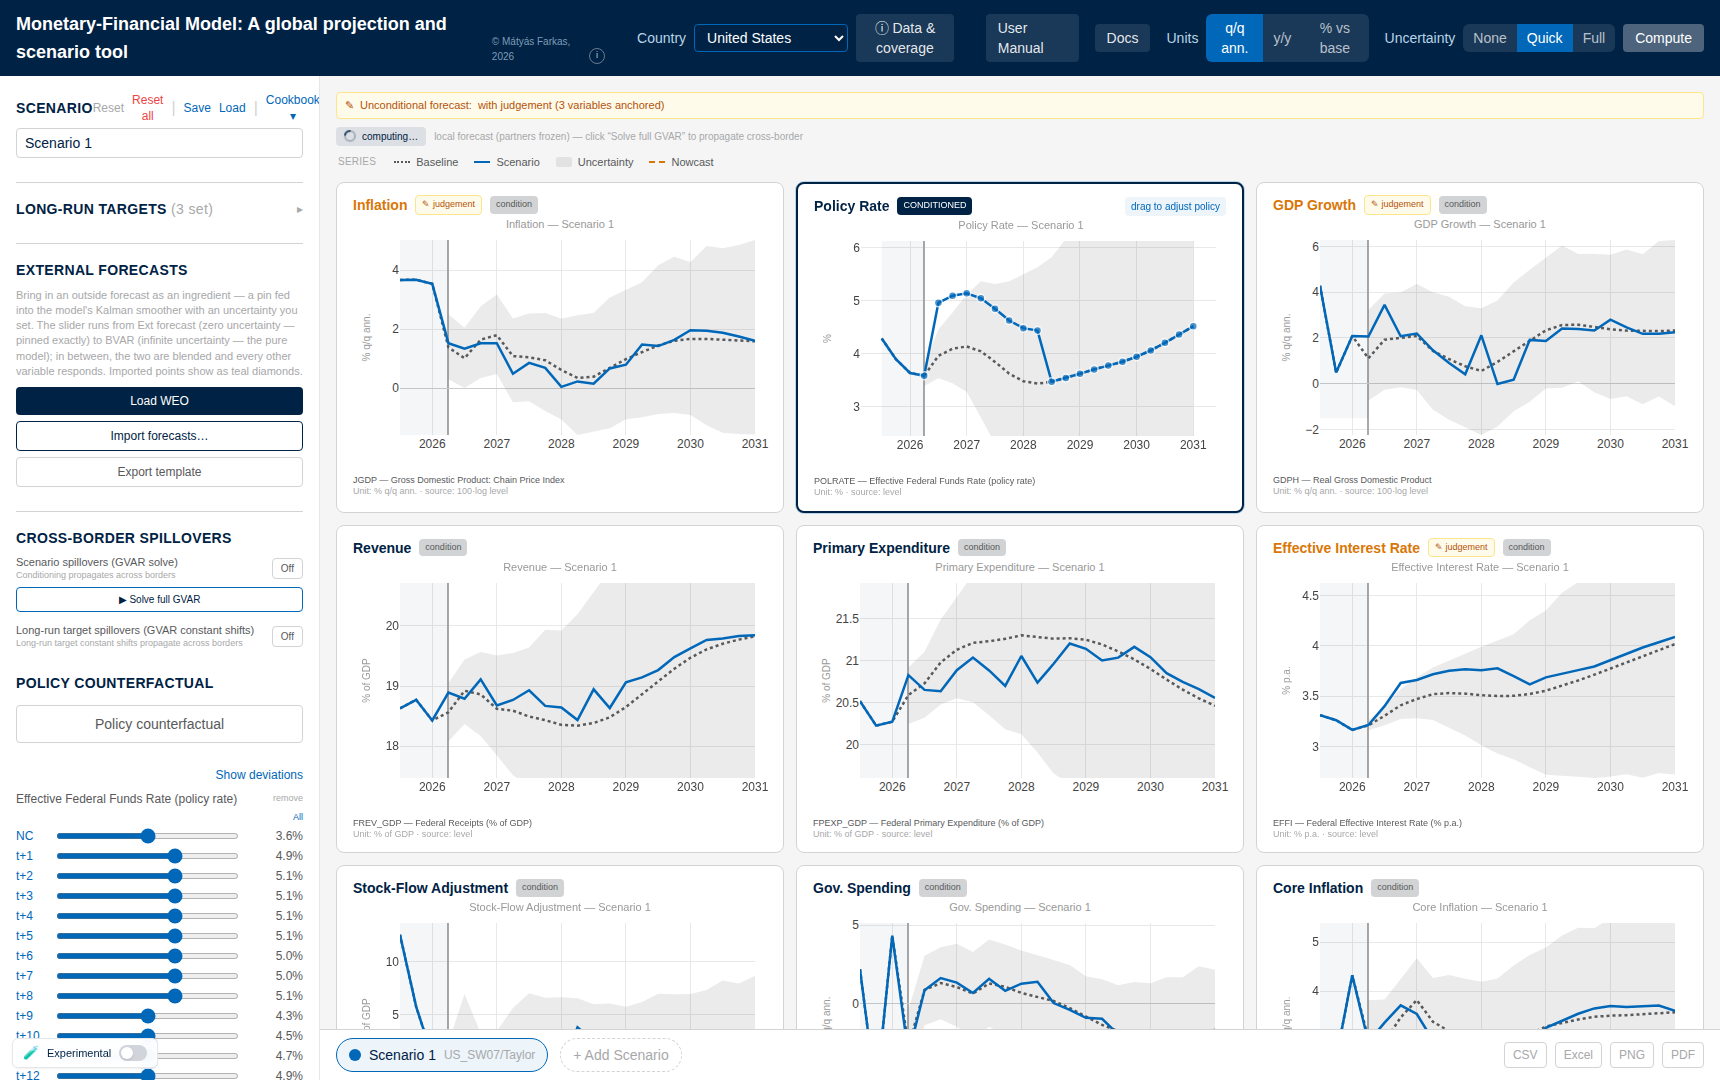
\includegraphics[width=0.98\textwidth]{../manual_figs/ui_conditioning.png}
\caption{The tool during conditioning, US bloc. Each panel shows history, the baseline
(dotted), the scenario (solid), and the uncertainty band; the highlighted panel carries the
user's pins, and every other panel updates as they are placed. The left rail holds the
scenario controls: long-run targets, external forecasts, the cross-border solve, and the
policy counterfactual. Interface view from an earlier release; the layout is unchanged.}
\label{fig:ui-cond}
\end{figure}

% Figure: one pin vs two pins — deviations from baseline, US bloc, display space.
% Data: figs/data/us_spread.csv (generated by app/scripts/paper_figs/us_spread_cf.mjs).
\begin{figure}[t]
\centering
\begin{tikzpicture}
\begin{groupplot}[
  group style={group size=3 by 2, horizontal sep=1.35cm, vertical sep=1.5cm},
  paperpanel,
]
\nextgroupplot[title={Baa corporate yield (pp)},
  legend style={font=\scriptsize, draw=none, fill=none, at={(0.95,0.95)}, anchor=north east}]
\addplot[zeroline] coordinates {(1,0)(20,0)};
\addplot[naiveline] table[x=q, y=baa_n, col sep=comma] {figs/data/us_spread.csv};
\addplot[trueline]  table[x=q, y=baa_t, col sep=comma] {figs/data/us_spread.csv};
\legend{one pin, two pins}
\nextgroupplot[title={10-year Treasury yield (pp)}]
\addplot[zeroline] coordinates {(1,0)(20,0)};
\addplot[naiveline] table[x=q, y=lr_n, col sep=comma] {figs/data/us_spread.csv};
\addplot[trueline]  table[x=q, y=lr_t, col sep=comma] {figs/data/us_spread.csv};
\nextgroupplot[title={Policy rate (pp)}]
\addplot[zeroline] coordinates {(1,0)(20,0)};
\addplot[naiveline] table[x=q, y=pol_n, col sep=comma] {figs/data/us_spread.csv};
\addplot[trueline]  table[x=q, y=pol_t, col sep=comma] {figs/data/us_spread.csv};
\nextgroupplot[title={Real GDP growth (pp, q/q ann.)}]
\addplot[zeroline] coordinates {(1,0)(20,0)};
\addplot[naiveline] table[x=q, y=gdp_n, col sep=comma] {figs/data/us_spread.csv};
\addplot[trueline]  table[x=q, y=gdp_t, col sep=comma] {figs/data/us_spread.csv};
\nextgroupplot[title={Inflation, GDP deflator (pp)}]
\addplot[zeroline] coordinates {(1,0)(20,0)};
\addplot[naiveline] table[x=q, y=infl_n, col sep=comma] {figs/data/us_spread.csv};
\addplot[trueline]  table[x=q, y=infl_t, col sep=comma] {figs/data/us_spread.csv};
\nextgroupplot[title={2-year Treasury yield (pp)}]
\addplot[zeroline] coordinates {(1,0)(20,0)};
\addplot[naiveline] table[x=q, y=fcm_n, col sep=comma] {figs/data/us_spread.csv};
\addplot[trueline]  table[x=q, y=fcm_t, col sep=comma] {figs/data/us_spread.csv};
\end{groupplot}
\end{tikzpicture}
\caption{One pin is not a spread shock. Deviations from the baseline forecast after conditioning
the US bloc on a 100 basis point rise in the Baa corporate yield at the nowcast quarter. With
one pin (dashed), the model reads the rise as a broad tightening: the ten-year and two-year
Treasury yields and the policy rate rise with it, and output is largely unaffected. Adding a
single further condition, the ten-year yield unchanged on impact (solid), turns the same rise
into a credit-spread shock: the curve stays put, output contracts, and policy eases. Horizontal
axis: quarters from the nowcast.}
\label{fig:naivetrue}
\end{figure}


The dashed lines in Figure~\ref{fig:naivetrue} show what comes back, and it is not a credit
event. The ten-year Treasury yield is up \NaiveLrImpactBp{} basis points on impact, the policy
rate climbs \NaivePolPeakBp{} basis points at its peak, and output barely reacts. The user
asked for a spread shock and received a shock to the general level of interest rates.

Understanding why requires the central idea of conditional forecasting. The smoother does
not treat a pin as a cause but as an observation, and it answers a precise question: among all the futures the estimated model considers possible, which is the
most likely one in which the Baa yield sits 100 basis points above baseline next quarter
\citep{WaggonerZha1999}? In \USSampleT{} quarters of data, the corporate yield is rarely that
much higher on its own. It is higher when the whole yield curve is higher. So the most likely
world consistent with the pin is one of generally tighter financial conditions, and that is
the world the model delivers: government yields up, the policy rate up, the spread between
corporate and government yields barely changed. The model did exactly what it was asked. The
user asked the wrong question.

\subsection{Two pins make a risk shock}\label{sec:truespread}

The fix costs one more click. Pin the ten-year government yield to stay at its baseline value
in the same quarter (not lower, not higher, simply unchanged) and solve again. The only
futures the smoother may now consider are those in which the corporate yield rises while the
risk-free curve stands still, and in the data those are the episodes in which credit risk is
being repriced.

The solid lines in Figure~\ref{fig:naivetrue} show the difference. The spread now opens by
the full 100 basis points. Output falls, with growth dipping \TrueGdpGrowthMinPp{} percentage
points below baseline at its worst and the level of GDP bottoming out \TrueGdpTroughPct{}
percent below baseline in quarter \TrueGdpTroughQ. Inflation drifts down, and the policy rate
eases, because in the estimated data that is what the Federal Reserve does when credit
tightens and activity weakens. None of this was imposed. Two numbers were pinned; the other
thirty-eight variables of the US bloc, every quarter of them, came from the model.

The episode carries two lessons. A scenario is defined as much by what you hold still as by
what you move, so the craft lies in fitting the pins to the story, and stories need fewer
pins than users expect. The second lesson is that the fiscal consequences arrive without
any extra work: the recession lowers revenue
and raises the debt ratio through the budget identity \eqref{eq:debt}, leaving debt
\DebtGapHPp{} percentage points of GDP above baseline after five years. The debt line moved
because accounting moved it, and it sits on the same screen as everything else.

The external accounts follow the same way, from the balance-of-payments identity in place of
the budget one. Each bloc is pinned by two real, sourced numbers: the net international
investment position at the start---for the United States, \ExtUsNfaSeed{} percent of GDP---and
the current account itself, taken from its published value. The bloc's estimated exports and
imports then supply only the \emph{deviations} from that anchor, and the net position rolls
forward by the balance-of-payments identity. Anchoring the level is what keeps the accounts
honest: a current account built from real-volume net exports alone comes out wrong, and for
several economies wrong in sign, once relative prices sit away from the chain-link reference.
The tool therefore never reports that raw level, and it suppresses the few very-open blocs
whose real-trade forecast would drive an implausible path. At the nowcast the current account
is its
published value---\ExtUsCaAnchor{} percent of GDP for the United States, a surplus of
\ExtEaCaAnchor{} percent for the euro area and \ExtCnCaAnchor{} percent for China.

Figure~\ref{fig:external} traces what the credit-spread scenario does to them: the recession
compresses imports faster than exports, so the current account improves by up to
\ExtScenCaPeakPp{} percentage points and the net-IIP ratio ends \ExtScenNfaDevH{} points above
baseline at the five-year horizon as the stronger balance rebuilds the stock. The deviations do
come from \emph{real}
trade, so a large terms-of-trade move would bias them---a channel to sharpen, not to distrust,
now that the level is anchored to the sourced figure.

% Figure: external-balance satellite — baseline vs credit-spread scenario, US bloc.
% Data: figs/data/us_external.csv (generated by app/scripts/paper_figs/nfa_pilot.mjs).
\begin{figure}[t]
\centering
\begin{tikzpicture}
\begin{groupplot}[
  group style={group size=2 by 1, horizontal sep=1.6cm},
  paperpanel,
]
\nextgroupplot[title={Current account (\% of GDP)},
  legend style={font=\scriptsize, draw=none, fill=none, at={(0.95,0.05)}, anchor=south east}]
\addplot[naiveline] table[x=q, y=ca_base, col sep=comma] {figs/data/us_external.csv};
\addplot[trueline]  table[x=q, y=ca_scen, col sep=comma] {figs/data/us_external.csv};
\legend{baseline, scenario}
\nextgroupplot[title={Net IIP / GDP (\%)}]
\addplot[naiveline] table[x=q, y=nfa_base, col sep=comma] {figs/data/us_external.csv};
\addplot[trueline]  table[x=q, y=nfa_scen, col sep=comma] {figs/data/us_external.csv};
\end{groupplot}
\end{tikzpicture}
\caption{External-balance satellite: the credit-spread scenario's consequence for the US external
accounts. Baseline (dashed) and two-pin scenario (solid) paths for the current account and the net
international investment position, in percent of GDP. The current account is \emph{anchored} to its
real published value at the nowcast and moves only by the model's real net-export deviation; the net
IIP is seeded from its real observed value and rolled forward by the balance-of-payments identity,
neither estimated. The scenario improves the current account as the recession compresses imports, and
the net-IIP ratio ends above baseline as the stronger balance rebuilds the stock. Horizontal axis:
quarters from the nowcast.}
\label{fig:external}
\end{figure}


\subsection{The global response}\label{sec:globalsolve}

So far the rest of the world has been standing still. That was the point of working in a
single bloc --- the US model carries its own reduced-form view of its partners --- and it is
exactly what the global solve corrects. One button re-solves the same two-pin scenario as a
fixed point of all \NBlocs{} blocs at once, through the pre-computed operator of
Section~\ref{sec:solve}, and the answer arrives in about a second. Every economy in the
dropdown now shows its own response, with the fiscal and external blocks derived alongside
(Figure~\ref{fig:ui-ea} shows the euro-area screen).

\begin{figure}[t]
\centering
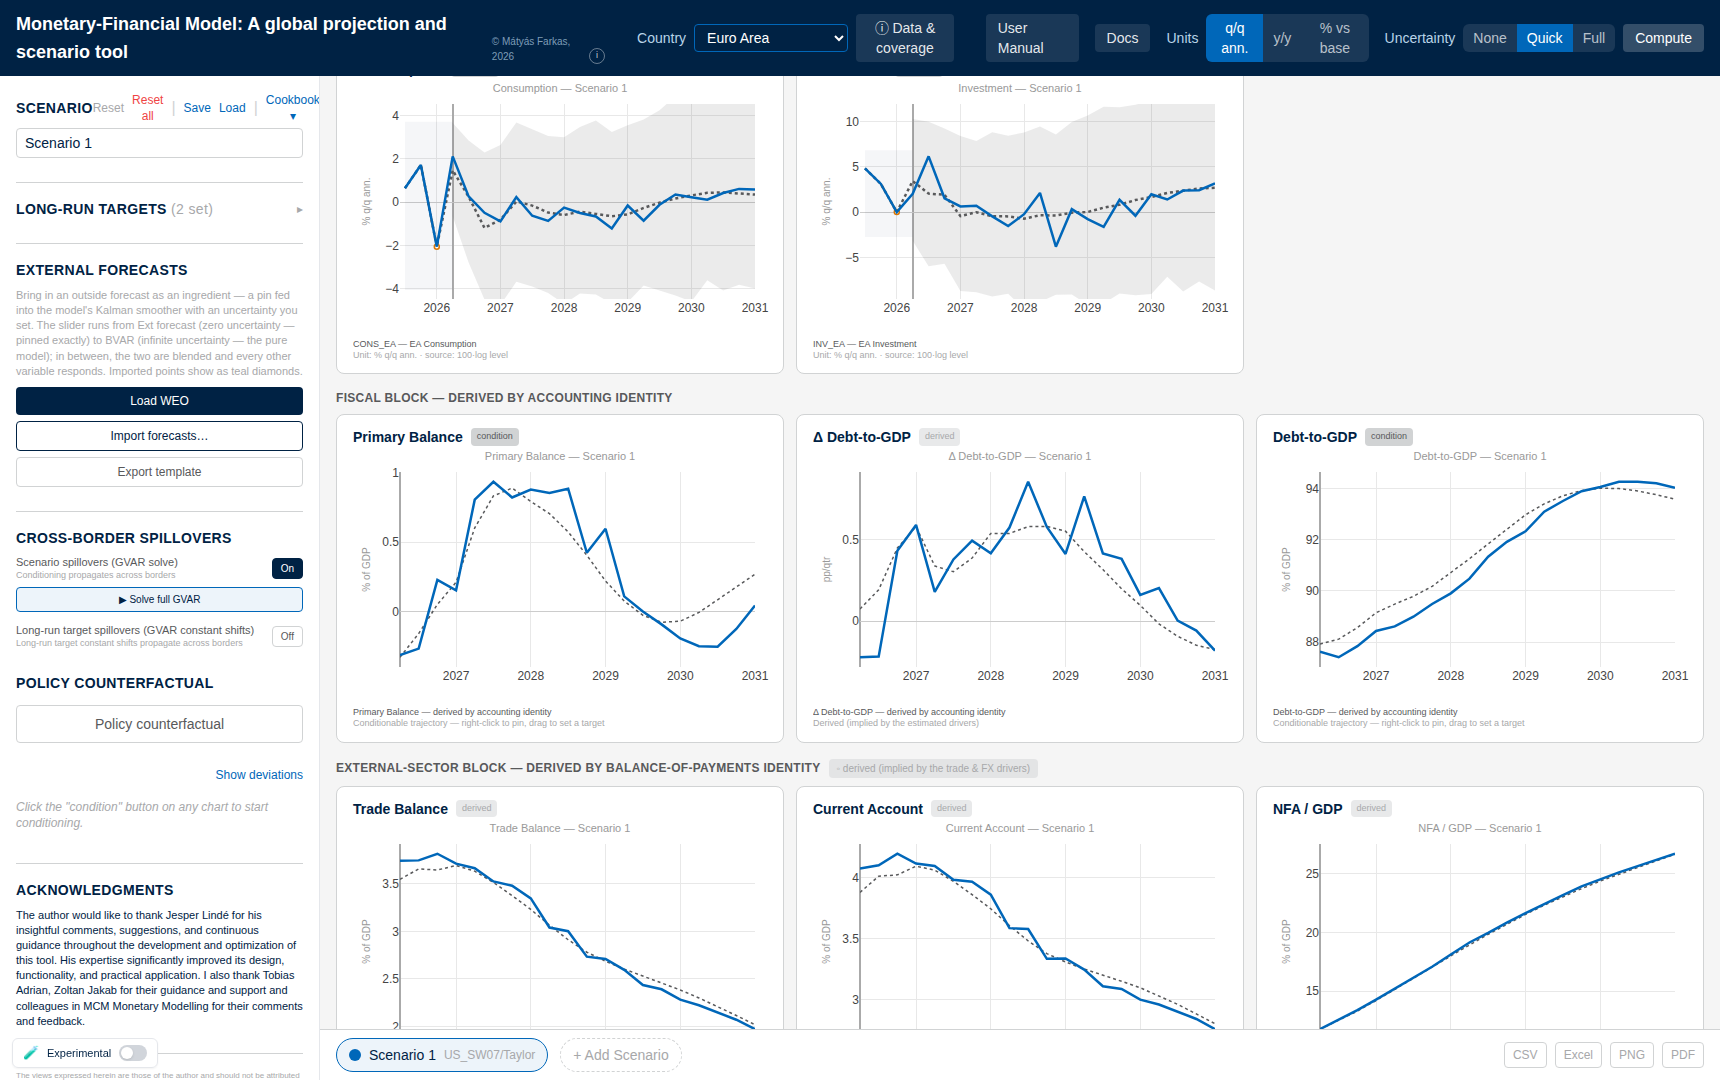
\includegraphics[width=0.98\textwidth]{../manual_figs/ui_gvar_ea.png}
\caption{The euro-area screen with cross-border spillovers switched on. The scenario was
built in the US bloc; the euro-area paths shown here come from the coupled solve. The lower
rows are not estimated: the fiscal block follows from the budget identity \eqref{eq:debt}
and the external block from the balance-of-payments identity, so a scenario's debt and
current-account consequences appear without further input. Interface view from an earlier
release; the layout is unchanged.}
\label{fig:ui-ea}
\end{figure}

% Figure: the spread shock through the global solve — GDP growth deviations.
% Data: figs/data/global_spread.csv, figs/data/world.csv (app/scripts/paper_figs/global_spread.mjs).
\begin{figure}[t]
\centering
\begin{tikzpicture}
\begin{groupplot}[
  group style={group size=2 by 2, horizontal sep=1.5cm, vertical sep=1.6cm},
  paperpanel, width=0.46\textwidth, height=0.30\textwidth,
]
\nextgroupplot[title={United States},
  legend style={font=\scriptsize, draw=none, fill=none, at={(0.95,0.05)}, anchor=south east}]
\addplot[zeroline] coordinates {(1,0)(20,0)};
\addplot[usoline]   table[x=q, y=us_uso,   col sep=comma] {figs/data/global_spread.csv};
\addplot[globline]  table[x=q, y=us_glob,  col sep=comma] {figs/data/global_spread.csv};
\addplot[jointline] table[x=q, y=us_joint, col sep=comma] {figs/data/global_spread.csv};
\legend{US bloc alone, global solve, spreads in US+EA+JP}
\nextgroupplot[title={Euro area}]
\addplot[zeroline] coordinates {(1,0)(20,0)};
\addplot[globline]  table[x=q, y=ea_glob,  col sep=comma] {figs/data/global_spread.csv};
\addplot[jointline] table[x=q, y=ea_joint, col sep=comma] {figs/data/global_spread.csv};
\nextgroupplot[title={Japan}]
\addplot[zeroline] coordinates {(1,0)(20,0)};
\addplot[globline]  table[x=q, y=jp_glob,  col sep=comma] {figs/data/global_spread.csv};
\addplot[jointline] table[x=q, y=jp_joint, col sep=comma] {figs/data/global_spread.csv};
\nextgroupplot[title={World}]
\addplot[zeroline] coordinates {(1,0)(20,0)};
\addplot[usoline]   table[x=q, y=w_uso,   col sep=comma] {figs/data/world.csv};
\addplot[globline]  table[x=q, y=w_glob,  col sep=comma] {figs/data/world.csv};
\addplot[jointline] table[x=q, y=w_joint, col sep=comma] {figs/data/world.csv};
\end{groupplot}
\end{tikzpicture}
\caption{The same shock, three ways. Real GDP growth deviations (pp, q/q annualized) under the
US credit-spread scenario of Figure~\ref{fig:naivetrue}. The dotted line solves the US bloc on
its own, so the rest of the world stays at baseline by construction and world output moves only
through the US share. The solid line runs the full coupled solve: the shock travels to the euro
area and Japan through trade and financial prices, and their responses feed back. The dashed
line imposes the same credit repricing in the United States, the euro area, and Japan at once.
World output is the GDP-weighted aggregate over the coupled blocs, using the tool's world
weights.}
\label{fig:global}
\end{figure}


Figure~\ref{fig:global} shows what changes, and the first thing to understand is \emph{how}
the shock travels, because it moves through two channels of different weight. The quieter
channel is trade: weaker US demand reaches the partners through their foreign variables, and
their weakness feeds back into the US stars, deepening the US growth trough from
\TrueGdpGrowthMinPp{} percentage points on its own to \USGdpTroughGlobPp{} in the coupled
solve. The
louder channel is financial. The two variables we pinned are the model's global financial
prices, carried by every bloc, so in the coupled solve the euro area and Japan face the same
credit repricing the United States does, directly in their own equations. A US credit event
is a world credit event in this model, by design rather than by accident, and the responses
show it: euro-area growth troughs \EAGdpTroughPp{} percentage points below baseline,
comparable to the US's own, and Japan deeper still at \JPGdpTroughPp{}.

The world panel puts the two solves side by side. Treated as a US-only event, world growth
dips \WorldTroughUsoPp{} percentage points at its trough, which is simply the US decline
scaled by its share of world output. The coupled solve deepens the world trough to
\WorldTroughGlobPp{} percentage points, about \WorldTroughRatio{} times as much. That gap is what a
country-by-country analysis leaves out, and a tool without a coupled global solve cannot
draw the second line at all.

One qualification belongs with these magnitudes. Most of the gap between the two lines is
definitional rather than estimated: the two pinned variables are global prices that every bloc
carries in its own equations, so imposing them on the euro area and Japan is close to imposing
the shock itself, and troughs of the same order as the US's own follow largely by
construction. The
genuinely estimated cross-border linkage is the quieter trade channel, which on its own deepens
the US trough only from \TrueGdpGrowthMinPp{} to \USGdpTroughGlobPp{} percentage points. The
coupled solve's contribution here is internal consistency and speed across \NBlocs{} blocs, not a
measurement of international transmission --- separating the common-price shock from its
propagation would require an identification this descriptive exercise does not attempt.

The third line answers a question that comes up in every stress-testing exercise: what if
the repricing is not only an American event? Imposing the same two-pin credit shock
simultaneously in the United States, the euro area, and Japan deepens the world trough
further, to \WorldTroughJointPp{} percentage points. Each economy now imports weakness from
the others while generating its own, which is the configuration financial-stability
exercises worry about. It takes six pins to build.

\subsection{What should policy do?}\label{sec:counterfactual}

Everything so far answers one kind of question: what is likely to happen. A policymaker's
next question is of a different kind: what should we do about it? Conditioning cannot answer
it. The smoother re-weights futures by likelihood; it does not identify cause and effect, and
``the world in which the central bank cuts'' is not the same object as ``the effect of a
cut'' \citep{AntolinDiazPetrellaRubioRamirez2021}. For the second object the tool carries a
structural layer: the policy-counterfactual option takes impulse responses from a fully
specified DSGE model (here \citealp{SmetsWouters2007}, from the Macroeconomic Model Data Base
of \citealp{WielandCwikMuellerSchmidtWolters2012}) and lays the model-implied effect of a
deliberate policy shock on top of the scenario.

% Figure: the SW07 policy counterfactual sized to offset the GDP trough.
% Data: figs/data/us_cf.csv (app/scripts/paper_figs/us_spread_cf.mjs).
\begin{figure}[t]
\centering
\begin{tikzpicture}
\begin{groupplot}[
  group style={group size=2 by 1, horizontal sep=1.6cm},
  paperpanel, width=0.46\textwidth, height=0.32\textwidth,
]
\nextgroupplot[title={Real GDP (\% deviation from baseline)},
  legend style={font=\scriptsize, draw=none, fill=none, at={(0.95,0.05)}, anchor=south east}]
\addplot[zeroline] coordinates {(1,0)(20,0)};
\addplot[trueline] table[x=q, y=gdp_scen_lvl, col sep=comma] {figs/data/us_cf.csv};
\addplot[cfline]   table[x=q, y=gdp_cf_lvl,   col sep=comma] {figs/data/us_cf.csv};
\legend{spread scenario, with policy response}
\nextgroupplot[title={Policy rate (pp deviation from baseline)}]
\addplot[zeroline] coordinates {(1,0)(20,0)};
\addplot[trueline] table[x=q, y=pol_scen, col sep=comma] {figs/data/us_cf.csv};
\addplot[cfline]   table[x=q, y=pol_cf,   col sep=comma] {figs/data/us_cf.csv};
\end{groupplot}
\end{tikzpicture}
\caption{What should policy do? The credit-spread scenario (solid) and the same scenario with
an unanticipated monetary-policy shock from the Smets--Wouters model layered on top (dashed),
sized so that the easing offsets the output trough. Left: the level of real GDP relative to
baseline; the counterfactual closes the gap the shock opened. Right: the policy-rate paths. The
scenario's own rate falls because the model expects policy to respond; the counterfactual adds
the deliberate surprise easing on impact, which then decays along the model's policy rule.}
\label{fig:cf}
\end{figure}


\begin{figure}[t]
\centering
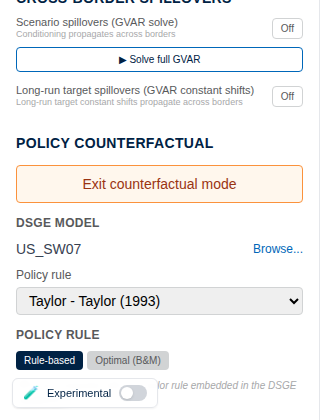
\includegraphics[width=0.34\textwidth]{../manual_figs/ui_cf_controls.png}
\caption{The policy-counterfactual controls. The user picks the DSGE model (here
Smets--Wouters, US\_SW07) and the policy rule from the Macroeconomic Model Data Base, enters
counterfactual mode, and sets the policy shock; the counterfactual is drawn as its own line
on every chart, labeled with the model that produced it. Interface view from an earlier
release.}
\label{fig:ui-cf}
\end{figure}

We ask a sharp version of the policy question: how large an unanticipated easing at the
nowcast quarter would undo the scenario's output loss at its trough? The tool back-solves
the required shock --- in the interface, through the controls of Figure~\ref{fig:ui-cf} ---
and the answer is \CFEasingBp{} basis points. Figure~\ref{fig:cf} shows the result: the easing closes the GDP gap at the trough (left panel), and the policy rate
jumps down on impact and then decays back along the Smets--Wouters policy rule (right
panel), sitting below the scenario's own rate path throughout.

The size of that number is itself the finding. The scenario's rate path already eases, since
the estimated model expects policy to respond to a credit tightening; the counterfactual asks
for the \emph{additional}, deliberate surprise that would fully offset the output trough,
delivered in a single quarter. A one-off surprise is an inefficient instrument against a
shock whose damage peaks a year out: its effect on output decays from the moment it lands,
so offsetting a one-percent output loss takes several hundred basis points up front. A
policymaker reading Figure~\ref{fig:cf} learns something concrete: against this scenario,
a realistic response is either persistent rather than one-off, or it accepts part of the
loss. Both variants are one click away in the tool, which is the point of having the layer
interactive.

The last thing this experiment teaches is a boundary, and we want to state it plainly. The
scenario layer is reduced-form: it says what tends to happen, given history, when spreads
widen. The policy layer is structural: it says what a specific model implies a deliberate
policy action does. The tool keeps the two visibly separate (the counterfactual is drawn as
its own line, labeled with the DSGE model that produced it) because conflating them is the
oldest mistake in applied macro. Appendix~B returns to this distinction in more detail.

% =====================================================================================
\section{Outside forecasts, long-run anchors, and policy overlays}\label{sec:toolkit}
% =====================================================================================

The worked example used only part of the platform, and the parts it did not use are the ones
that connect the tool most directly to how forecasting is actually practiced in policy
institutions. Institutional forecasts are never purely model output: they blend the model
with outside forecasts, with views about where the economy settles in the long run, and with
structural reasoning about deliberate policy choices. The MFFM carries a device for each of
these, and because each one works through the same estimated model and the same smoother,
the blended forecast remains a single coherent object rather than a collage. This section
explains how the three devices work, in enough detail that a reader could predict what each
one will do before touching it.

\subsection{Outside forecasts as soft conditions}\label{sec:soft}

A desk economist rarely faces a blank slate. There is a WEO projection, a consensus number,
or the desk's own view, and the practical question is never whether to use it but how much
weight it should carry against the model. The tool answers that question with the one
parameter the smoother already understands: measurement error. Recall from
Section~\ref{sec:solve} that a scenario pin is treated as a future observation of the model,
\begin{equation}\label{eq:softpin}
  y^{\mathrm{pin}}_{j,t+h} \;=\; \bigl(Z\alpha_{t+h}\bigr)_j + \varepsilon_{j,t+h},
  \qquad \varepsilon_{j,t+h}\sim\mathcal N(0,\,R_{j,h}),
\end{equation}
and that a hard pin sets the variance $R_{j,h}$ essentially to zero, so the smoother matches
the imposed value exactly. An outside forecast enters through exactly the same equation with
a finite variance, chosen by a dial that runs from ``impose exactly'' to ``ignore
entirely.'' In between, the smoother forms the precision-weighted compromise between the
outside number and the model's own predictive distribution, quarter by quarter, and every
other variable in the system adjusts in proportion to how far the compromise moved. The
device is the stochastic conditioning of \citet{WaggonerZha1999} put behind a single slider,
and its interpretation is exactly Bayesian: the outside forecast is data about the future,
observed with an error whose size expresses how much the user trusts its source. Feed in a
WEO path for US growth at high trust and the whole US bloc --- and, through the solve of
Section~\ref{sec:solve}, the world --- re-forms around it; lower the trust and the forecast
relaxes back toward the model, continuously. Because imported paths are marked on the
charts, a reader of the resulting scenario can always see which parts of it came from
outside and how strongly they were held.

\subsection{Long-run anchors}\label{sec:anchors}

Users often know more about the destination than about the journey: the inflation target,
an estimate of potential growth, a view on the neutral rate. The natural econometric home
for such knowledge is Villani's steady-state parametrization of the VAR
\citep{Villani2009}, in which the modeler places an informative prior directly on the
long-run mean and the estimated dynamics carry the forecast toward it. The MFFM implements
the reactive counterpart of that idea: the user states the long-run value --- inflation at
two percent, say --- and the forecast is re-centered on it after estimation, so the device
responds in seconds when the user changes her mind about the destination, with no
re-estimation and no new draws. The mechanics respect the model's own dynamics. The stated
long-run value fixes the terminal displacement of the anchored variable, and that
displacement is phased in along the model's convergence profile,
\begin{equation}\label{eq:anchor}
  \Delta y_{j,t+h} \;=\; w_j(h)\,\Delta^{*}_{j}, \qquad
  w_j(h)=\frac{S_h[j,j]}{S_H[j,j]}, \qquad
  S_h=\textstyle\sum_{k=0}^{h-1}\mathbf T^{\,k},
\end{equation}
where $\mathbf T$ is the companion matrix of Section~\ref{sec:estimation} and
$\Delta^{*}_{j}$ the terminal shift that lands the variable on its stated value. The weight
$w_j(h)$ starts at essentially zero and accumulates to one at exactly the speed with which
the model itself propagates a sustained change, so the near-term forecast is left
untouched, there is no jump at the forecast origin, and the path glides to its new steady
state neither faster nor slower than the estimated dynamics allow. The exact infinite-horizon
steady state is not available here --- under a prior centered on random walks the long-run
matrix is near-singular --- which is why the finite-horizon profile $S_h/S_H$ stands in for
the classical $(I-\mathbf T)^{-1}$ and makes the device well defined for every bloc. A
legacy alternative, a parallel shift that imposes the full adjustment from the first
quarter as a constant drift, survives as a settings toggle, but the steady-state transition
is the default and the shape users see. Uncertainty bands are unaffected, since the device
moves the mean and nothing else; in the seasonal blocs the re-centering is applied
identically across the four quarterly intercepts, so the anchor targets the seasonally
adjusted path and leaves the seasonal pattern alone. Anchors can be set per variable or
jointly, and the shipped defaults --- official targets and consensus long-run values ---
are the ones the evaluation of Appendix~\ref{app:cred} examines as a forecasting device in
their own right.

\subsection{The policy overlay: a DSGE delta on a reduced-form world}\label{sec:overlay}

The counterfactual of Section~\ref{sec:counterfactual} rests on a division of labor that
deserves to be stated precisely, because it is the platform's answer to the oldest
objection to reduced-form policy analysis. The estimated model supplies the world: the
scenario, with everything it implies, is a statement about likelihoods under the policy
behavior embedded in the data. What the estimated model cannot supply is the effect of a
\emph{deliberate departure} from that behavior --- that is a causal object, and for it the
tool turns to a structural model. The user selects a DSGE model and a policy rule from the
Macroeconomic Model Data Base \citep{WielandCwikMuellerSchmidtWolters2012}; the platform
ships the model's impulse responses to an unanticipated policy shock. When the user
specifies a rate adjustment --- a path, or a single surprise at one quarter --- the layer
back-solves the sequence of policy shocks that delivers exactly that adjustment under the
chosen model's rate response, by inverting the convolution
\begin{equation}\label{eq:delta}
  \Delta r_{t+h} \;=\; \textstyle\sum_{k\le h}\, \phi^{\,r}_{h-k}\,\eta_k,
\end{equation}
where $\phi^r$ is the rate's impulse response and $\eta$ the shock sequence; the same
shocks, run through the model's responses for inflation and output, give the deltas for
those variables. The deltas are then laid on top of the scenario paths --- inflation
accumulated into the price level, the output gap applied as a level deviation, conventions
that matter and are easy to get wrong --- and the smoother is run once more with these
paths imposed, so that the remaining thirty-odd variables of the bloc adjust coherently
around the structural core. The counterfactual appears as its own line, labeled with the
model that produced it. The logic is a delta method: only the marginal effect of the
deliberate policy surprise is asked of the structural model, which is precisely the piece
the reduced-form scenario cannot identify, while everything the data speak to --- the
baseline, the scenario, the co-movements --- stays with the estimated model. Different DSGE
models give different deltas, and the tool makes switching between them a one-click
sensitivity check rather than a research project.

% =====================================================================================
\section{Conclusion}\label{sec:conclusion}
% =====================================================================================

What does the tool give an economist today? A morning's question --- credit has repriced,
what does it mean, what should we do --- became, in Section~\ref{sec:example}, two pins, one
button, and one structural overlay: a globally consistent scenario for \NModels{} economies,
its fiscal arithmetic included, and a priced policy response, all inside an hour that used to
be a memo requesting a model run. The scenario-analysis literature of
Section~\ref{sec:intro} presumes that coherent scenarios and reference forecasts exist and
can be produced on demand; the MFFM is the machine that produces them, on any desk.

Around the example and the toolkit sits the practical machinery a working instrument needs:
scenarios export to spreadsheets and to a session file that reloads with one click on a
colleague's screen, and the online manual documents every convention this paper has touched.

These capabilities line up, deliberately, with the steps of an institutional projection
round. The ECB's account of forecasting with its multi-country model
\citep{AngeliniBokanCiccarelliLalikZimic2025} decomposes the process into assessing the
impact of external assumptions, updating the projection on new data, layering judgment
through add-factors, and decomposing the revision for communication. The MFFM carries a
disciplined analogue of each step: assumptions enter as conditioning paths, hard or soft;
the projection updates through a data shift that re-anchors every forecast while the model
stays fixed; judgment enters through the long-run anchors and the trust dial on outside
forecasts, devices with stated mechanics rather than free add-factors; and a release-impact
monitor records what each new quarter changed, bloc by bloc. An economist who knows the
projection workflow will find its stations here, compressed from a committee cycle into a
browser session.

Two lines of work come next. The out-of-sample forecast evaluation --- the tool's model
against the random walk, univariate autoregressions, a closed-economy Bayesian VAR, the
classical GVAR, and a Bayesian GVAR in the manner of \citet{CrespoFeldkircherHuber2016}, in the
tradition of \citet{AdolfsonLindeVillani2007} --- has been restarted
on the current vintage and will be reported in a companion paper. And the structural layer
invites extension: generalized impulse responses and connectedness measures for the coupled
system, and a broader menu of policy experiments from the model data base. The platform is
built to absorb both without changing what a user already knows.

% =====================================================================================
\appendix
\section{Model detail}\label{app:model}

Section~\ref{sec:method} carries the model itself; this appendix records the pieces a
replicator needs beyond it.

\paragraph{The prior, exactly.} Stacking bloc $i$'s coefficients as
$\beta_i=(c_i,\Gamma_i,B_{i1},\dots,B_{ip})'$, the conjugate prior is
$\Sigma_i\sim\mathcal{IW}(\Psi_i,\,d_i)$ and
$\mathrm{vec}(\beta_i)\,|\,\Sigma_i\sim\mathcal N\!\bigl(\mathrm{vec}(b_i),\,\Sigma_i\otimes\Omega_i\bigr)$,
with $b_i$ the random-walk mean (own first-lag one; zero on the fiscal-ratio columns), and
$\Omega_i$ diagonal with entries $\lambda_i^2/(\ell^2\psi_j)$ for the coefficient on lag
$\ell$ of variable $j$, following \citet{Giannone2015}. The scales $\psi_j$ are fixed at
univariate AR residual variances; the intercept and seasonal-dummy rows carry a diffuse
variance. The sum-of-coefficients prior enters as the dummy observations of
\citet{DoanLittermanSims1984} with tightness $\mu_i$; on seasonal blocs the dummy
observations carry zeros in the $D_t$ columns. Hyperpriors: $\lambda_i\sim$ Gamma with mode
$0.2$ and standard deviation $0.4$; $\mu_i\sim$ Gamma with mode $1$ and standard deviation
$1$; both updated by random-walk Metropolis--Hastings on the completed-data marginal
likelihood, proposals reflected into $[10^{-4},5]^2$. The estimator is
\code{cgl\_bvarV5.m} in the tool's repository, driven by
\code{export\_bvar\_gvar24\_loop.m}.

\paragraph{The operator $M$.} An entry of $M$ answers one question: if partner $j$'s solved
level paths deviate from baseline by one unit in one cell, by how much does bloc $i$'s star
path deviate? The star definitions \eqref{eq:rowdem}--\eqref{eq:rowfin} make the map from
partner paths to star paths linear with weights \eqref{eq:wtilde}; the bloc's
conditional-forecast operator (the smoother of \eqref{eq:ss} with pinned stars) is affine;
composing the two over all bloc pairs, horizon step by horizon step, fills $M$. Four extra
row blocks carry the US-originated global prices, which the US bloc's own solution
determines and every other bloc receives. The construction is
\code{buildLinearSystemEndo} in \code{gvarSolve.ts}; the export-time inverse is
\code{precompute\_gvar\_coupling.mjs}.

\paragraph{Algorithm fine print.} Within the outer iteration the smoother's companion is
held at the previous pass's posterior mean and common random numbers are reused across
passes, so successive passes differ only through the star data --- this is what makes the
outer loop contract in practice. An exact data-augmentation pass (companion rebuilt at
every Gibbs sweep) is available behind a flag as a final polish. Convergence is measured on
the star histories excluding the pandemic-imputation window, whose cells legitimately churn
across passes. The \NMembers{} euro-member satellites are estimated separately, each a
standalone BVAR whose euro-area columns are pinned at solve time to the EA bloc's solution.

\section{Credibility: testing, interpretation, and a classical-GVAR comparison}\label{app:cred}

A tool used for policy must show its work, and this appendix says how this one is tested,
how its output should and should not be read, and where its evaluation stands.

\paragraph{Testing.} The computation engine ships with an invariant test suite (about five
hundred tests) that runs on every change: the TypeScript smoother is cross-validated
against the MATLAB reference implementation on the canonical conditional forecast; the
closed-form global solve is verified against the iterative fixed point; the seasonal
forecast path produced by the filter and by the band simulator agree to numerical
precision; and a deterministic-mean canary pins the shipped baselines to the estimation
output. Data provenance travels with the data: every model-completed cell is flagged in
the interface, vintages are archived on every data shift, and a release-impact monitor
records what each new quarter changed. None of this substitutes for external review, which
we invite.

\paragraph{Interpretation.} A conditional forecast is a statement about likelihood, not
about cause: it re-weights the model's futures by consistency with the pins
\citep{WaggonerZha1999}, and only the structural layer of
Section~\ref{sec:counterfactual} makes causal claims, on the authority of the DSGE model
chosen there \citep{AntolinDiazPetrellaRubioRamirez2021}. The distinction is kept visible
in the interface: the counterfactual is a separate line, labeled with its model.

\paragraph{The classical-GVAR confrontation.} The one quantitative credibility exhibit we
commit to in this paper is a same-data confrontation: a classical GVAR --- estimated with
the Smith--Galesi toolbox routines \citep{SmithGalesi2014} on the balanced window the
classical recipe requires --- subjected to the US credit-spread experiment, its generalized
impulse responses \citep{PesaranShin1998} set against the tool's conditional deltas of
Section~\ref{sec:example}. The exhibit is being produced with the restarted evaluation
(below) and will appear in this appendix in the next revision.

\paragraph{A Bayesian-GVAR head-to-head.} The nearest relative of our estimator is the
Bayesian GVAR of \citet{CrespoFeldkircherHuber2016}, and we ran the comparison in both
directions: their exercise replicated with their own archived code and data, and our
estimator run on a common public panel. Their finding survives both. On their 36-country
panel their code, at reduced posterior sampling over the same 2004--2013 hold-out,
reproduces the structure of their results: shrinkage is what separates a useful GVAR from
a useless one --- at the year horizon the no-shrinkage GVAR's relative RMSE on short rates
reaches \CcfhDiffuseStirHFour{} against \CcfhSzStirHFour{} under the Sims--Zha prior ---
and the shrunk model beats the univariate AR(5) benchmark on output, equity, long rates
and oil one quarter ahead. The working part is the prior family: a random-walk prior mean
with sum-of-coefficients and dummy-initial-observation dummies, tuned by marginal
likelihood --- the same family this tool's estimator carries
(Section~\ref{sec:method}). Run on the public 28-country \texttt{pesaranData} panel under
the same expanding-window design, our G-BVAR delivers the same qualitative verdict against
the AR(5) --- and the full exercise, carried to nine quarters ahead across nine models
with anchored and no-global-solve variants and a regional cut, is
Appendix~\ref{app:ccfhperf}, which mirrors their Section~4.3 paragraph by paragraph. The
package implementation of the Bayesian GVAR estimated at its
defaults --- a white-noise prior mean, no sum-of-coefficients dummies --- loses to the
AR(5) on every variable on the same panel. That is a caution about defaults, not about the
method: with the prior \citeauthor{CrespoFeldkircherHuber2016} actually use, their result
stands, and our estimator inherits it.

\paragraph{Forecast evaluation.} The out-of-sample evaluation has been restarted on the
current vintage, in the simplest form that answers the question: the tool's model, with
its seasonal treatment and with and without the shipped long-run anchors, against the
random walk, an AR(1), a closed-economy Bayesian VAR with the same prior, the classical
GVAR above, and the Bayesian GVAR of the head-to-head, across all coupled blocs --- the
benchmark tradition of \citet{AdolfsonLindeVillani2007}. A second leg will follow the design the ECB uses for its
own multi-country model \citep{AngeliniBokanCiccarelliLalikZimic2025}: condition on the
\emph{realized} financial and external paths and ask how well the model translates correct
assumptions into macro forecasts, against a random-walk reference --- an exercise our
conditioning machinery performs natively --- illustrated on one narrative episode. A
four-origin pilot of the evaluation on the platform's own panel closes
Appendix~\ref{app:ccfhperf}; the full expanding-window results go to a companion paper ---
this one documents the platform.

% appendix_ccfh.tex — out-of-sample forecast performance on the CCFH design.
% Mirrors the structure of Crespo Cuaresma, Feldkircher and Huber's (2016) Section 4.3
% paragraph by paragraph, in their register. All numbers are generated by
% app/scripts/paper_figs/ccfh_matrix.mjs from the evaluation-repository results; an
% editorial pass (2026-07-24) verified every quantitative claim against the tables.

\section{Forecast performance on the CCFH design}\label{app:ccfhperf}

Two strands of literature meet in this exercise. The first studies Bayesian shrinkage as
the route to forecasting with vector autoregressions: from the Minnesota prior of
\citet{DoanLittermanSims1984} and \citet{Litterman1986} and the weighted combination of
its components in \citet{simszha1998}, through the demonstration by
\citet{BanburaGiannoneReichlin2010} that, with shrinkage tightened as the system grows,
very large systems forecast as well as small ones, to
\citet{Koop2013} and \citet{CarrieroClarkMarcellino2015} on specification and prior
choices in medium and large systems, \citet{Giannone2015} on setting the shrinkage
hyperparameters by marginal likelihood --- the tuning approach our estimator carries ---
and \citet{Clark2011} on the density side. The second asks whether modeling
international linkages pays: the GVAR of \citet{PesaranSchuermannWeiner2004} and
\citet{DeesDiMauroPesaranSmith2007} was first systematically evaluated out of sample by
\citet{PesaranSchuermannSmith2009}, who report gains over univariate benchmarks that are
present but uneven across variables and countries; \citet{GreenwoodNimmoNguyenShin2012}
extend the evaluation to probabilistic forecasts, \citet{HanNg2011} to a regional panel,
and \citet{DovernFeldkircherHuber2015} ask directly whether joint modeling of the world
economy improves multivariate forecasts. \citet{CrespoFeldkircherHuber2016} ---
henceforth CCFH --- join the two strands: Bayesian shrinkage estimated within a GVAR,
evaluated over a forty-quarter hold-out against univariate and non-shrinkage
alternatives, with the conclusion that the combination --- not either ingredient alone
--- delivers the improvement. Their design has become the reference for the class, and
this appendix adopts it; \citet{ChudikPesaran2016} survey the wider GVAR literature, and
\citet{AdolfsonLindeVillani2007} established the corresponding benchmark-suite tradition
for open-economy policy models.

The evaluation conventions are equally settled. Point accuracy is reported as root mean
squared error relative to a naive univariate benchmark, density accuracy as log
predictive scores --- the measure grounded in \citet{Geweke2001} and surveyed by
\citet{GewekeWhiteman2006}, with \citet{GewekeAmisano2010} on the comparison of
predictive distributions --- and differences in predictive accuracy are
assessed in the tradition of \citet{DieboldMariano1995} with the small-sample correction
of \citet{HarveyLeybourneNewbold1997}. Three questions recur across this literature
without resolution. Horizons beyond one year are rarely examined --- most GVAR
evaluations, CCFH included, stop at four quarters --- although the shrinkage priors at
issue are designed around low-frequency behavior. The respective contributions of the
prior and of the international linkages are confounded in every comparison that changes
both at once, as \citet{PesaranSchuermannSmith2009} and
\citet{CrespoFeldkircherHuber2016} do by construction. Finally, the information in
observable forward-looking data --- policy guidance, the yield curve --- enters none of
the standard specifications, although the hold-outs of this literature span the
effective-lower-bound years in which that information contradicted historical means most
sharply. The exercise below addresses all three: it extends the horizon grid to nine
quarters, holds the prior fixed while removing the linkages, and evaluates anchors built
from each origin's own term structure.

The evaluation design matches CCFH's in all but four respects, following their
Section~4.3 step by step. The initial estimation sample ends in 2003:Q4, and the 40 quarters
2004:Q1--2013:Q4 form the hold-out. Every model is re-estimated at each origin over an
expanding window. Point forecasts are evaluated by root mean squared error and density
forecasts by log predictive scores; all measures are benchmarked against a fifth-order
univariate autoregression. Four differences remain. First, where they consider one- and
four-quarter horizons, we evaluate every horizon up to nine and report $h=1$, $5$ and $9$
($h=1$ denotes the nowcast quarter, so $h=9$ corresponds to $t+9$ under origin-relative
dating). Second, where their panel is the 36-country, seven-variable dataset of
\citet{DovernFeldkircherHuber2015}, ours is the public 28-country \texttt{pesaranData}
panel with the six common variables (real output, inflation, short- and long-term
interest rates, the real exchange rate, and equity prices; total credit is not
available), and two lags rather than their five, which keeps the 40 re-estimations of 28
country models tractable. Third, we summarize by the cross-country median where their
tables report unweighted averages. Fourth, the \texttt{BGVAR} package runs at its default
prior hyperparameters --- with one stated exception: the eigenvalue truncation is raised
from 1.05 to 1.5, without which no SSVS draw survives on data in near-unit-root levels
--- whereas their specification tunes hyperparameters by marginal likelihood; their
published configuration is reproduced with their archived code and data in
Appendix~\ref{app:cred}. One further departure is common to both sides: the trade
weights are the package's 1980--2016 averages, where CCFH restrict weights to
1980--2003 to keep them real-time. The weights enter our leg and the package's leg
identically, so the head-to-head is unaffected, but neither leg is strictly real-time in
the weights. The two exercises therefore answer separate questions: this
one compares the estimators under identical conditions; that one asks whether their
published results can be reproduced.

\begin{table}[t]
\centering
\caption{Point-forecast accuracy on the CCFH design: relative RMSE against the AR(5)
benchmark, median across the 28 \texttt{pesaranData} countries (40 origins, 2004--2013,
re-estimated at every origin). A dagger marks cells whose summed log predictive score
exceeds that of the AR(5). ``+anch.''\ applies the long-run targets of
Section~\ref{sec:anchors}: drift targets for trending log-levels, the recursive
as-of-origin mean for inflation, and, for the interest rates, the forward-rate path
implied by each origin's own yield curve under the expectations hypothesis (see text). No
future information enters any target. The SSVS and MN columns run the \texttt{BGVAR}
package at default hyperparameters; RW is the last-observation random walk, point-scored
only.}
\label{tab:ccfhmatrix}
\footnotesize\setlength{\tabcolsep}{3pt}
\begin{center}
% GENERATED by app/scripts/paper_figs/ccfh_matrix.mjs — do not edit by hand.
\begin{tabular}{lcccccccc}
\toprule
 & G-BVAR & +anch. & no-solve & +anch. & cl.\ GVAR & SSVS & MN & RW \\
\midrule
\multicolumn{9}{l}{\emph{One quarter ahead (the nowcast, $h=1$)}} \\
\midrule
Output & 0.87$^{\dagger}$ & 0.89$^{\dagger}$ & 0.90$^{\dagger}$ & 0.91$^{\dagger}$ & 0.96$^{\dagger}$ & 1.85 & 1.90 & 1.10 \\
Inflation & 1.02$^{\dagger}$ & 1.07 & 1.01$^{\dagger}$ & 1.04 & 1.26 & 1.68 & 1.76 & 1.05 \\
Short rate & 0.95$^{\dagger}$ & 0.99$^{\dagger}$ & 0.99$^{\dagger}$ & 0.96$^{\dagger}$ & 1.60 & 6.24 & 10.50 & 0.97 \\
Long rate & 1.09 & 1.12 & 1.04 & 1.07 & 2.02 & 10.25 & 14.87 & 0.98 \\
Exch.\ rate & 0.99 & 0.97$^{\dagger}$ & 0.98$^{\dagger}$ & 0.96$^{\dagger}$ & 1.37 & 1.55 & 1.67 & 0.99 \\
Equity & 0.96$^{\dagger}$ & 1.05 & 0.95$^{\dagger}$ & 0.98$^{\dagger}$ & 2.37 & 1.57 & 1.67 & 1.01 \\
\addlinespace
\multicolumn{9}{l}{\emph{Five quarters ahead ($h=5$)}} \\
\midrule
Output & 0.75$^{\dagger}$ & 0.74$^{\dagger}$ & 0.76$^{\dagger}$ & 0.73$^{\dagger}$ & 1.85 & 1.21 & 1.00 & 0.98 \\
Inflation & 1.00$^{\dagger}$ & 1.18 & 0.98$^{\dagger}$ & 1.12 & 1.70 & 2.38 & 1.59 & 1.13 \\
Short rate & 0.85$^{\dagger}$ & 0.87$^{\dagger}$ & 0.89$^{\dagger}$ & 0.90$^{\dagger}$ & 2.52 & 3.11 & 3.51 & 0.84 \\
Long rate & 0.96$^{\dagger}$ & 1.14 & 0.90$^{\dagger}$ & 1.11 & 4.75 & 4.34 & 5.40 & 0.80 \\
Exch.\ rate & 0.90$^{\dagger}$ & 0.78$^{\dagger}$ & 0.86$^{\dagger}$ & 0.78$^{\dagger}$ & 2.65 & 0.96 & 0.88 & 0.78 \\
Equity & 0.87$^{\dagger}$ & 0.94 & 0.85$^{\dagger}$ & 0.91$^{\dagger}$ & 2.88 & 1.32 & 1.09 & 0.90 \\
\addlinespace
\multicolumn{9}{l}{\emph{Nine quarters ahead ($h=9$)}} \\
\midrule
Output & 0.64$^{\dagger}$ & 0.62$^{\dagger}$ & 0.62$^{\dagger}$ & 0.62$^{\dagger}$ & 1.50 & 1.15 & 0.87 & 0.93 \\
Inflation & 0.96$^{\dagger}$ & 1.12 & 0.95$^{\dagger}$ & 1.13 & 2.30 & 2.85 & 1.47 & 1.14 \\
Short rate & 0.72$^{\dagger}$ & 0.77$^{\dagger}$ & 0.80$^{\dagger}$ & 0.76$^{\dagger}$ & 1.83 & 2.41 & 2.37 & 0.76 \\
Long rate & 0.85$^{\dagger}$ & 1.06 & 0.78$^{\dagger}$ & 1.05 & 2.16 & 3.60 & 4.18 & 0.72 \\
Exch.\ rate & 0.79$^{\dagger}$ & 0.75$^{\dagger}$ & 0.81$^{\dagger}$ & 0.74$^{\dagger}$ & 2.45 & 0.93 & 0.77 & 0.73 \\
Equity & 0.84$^{\dagger}$ & 0.89 & 0.86$^{\dagger}$ & 0.90 & 4.23 & 1.36 & 1.01 & 0.86 \\
\bottomrule
\end{tabular}

\end{center}
\end{table}

\paragraph{Overall results, one quarter ahead.} Their one-quarter findings are threefold:
most specifications improve upon the naive benchmark in point forecasts; neither
country-specific shrinkage nor international linkages dominates when considered
separately; and combining the two improves forecast performance considerably. The first
panel of Table~\ref{tab:ccfhmatrix} confirms the first finding for our estimator: the
G-BVAR improves upon the benchmark for output (\CmGbvarYHOne{}), the short rate
(\CmGbvarRHOne{}) and equity prices, is at approximate parity for inflation and the
exchange rate (\CmGbvarDpHOne{} and 0.99), and underperforms only for the long rate. The
classical GVAR attains \CmToolboxYHOne{} for output but exceeds unity for the remaining
variables, and the package's ratios at default hyperparameters exceed unity everywhere
--- output \CmSsvsYHOne{} under SSVS, short rates \CmMnRHOne{} under the Minnesota prior
--- consistent with their observation that the conjugate prior without tuned shrinkage
performs least well, here in more extreme form. On the second and third findings our
design permits a sharper decomposition. Their comparison sets a country-specific BVAR
against a GVAR under a diffuse prior, so the prior and the linkages change together; ours
holds the prior fixed and removes only the foreign variables. The G-BVAR and
no-global-solve columns of Table~\ref{tab:ccfhmatrix} differ by at most
\CmStarsNostarsGap{} at any variable and horizon: conditional on the prior, the
international linkages contribute little to point accuracy on this panel. On this
evidence, the improvement they find from combining shrinkage with linkages owes primarily
to the shrinkage, which in their comparison arrives jointly with the linkages. The same
division of labor is why the platform justifies the coupled solve by cross-country
consistency rather than by forecast accuracy (Section~\ref{sec:example}).

\paragraph{Density forecasts.} Their density results confirm their point results, with
the largest improvements among the shrinkage GVARs. The same holds here: the sum over
countries of the G-BVAR's log-score differences relative to the AR(5) is
\CmGbvarYLpsHOne{} for output at the nowcast and \CmGbvarYLpsHNine{} at $h=9$ (the
corresponding cells carry daggers in Table~\ref{tab:ccfhmatrix}); the no-global-solve
column performs comparably; the package's densities are inferior throughout at default
hyperparameters. For the interest rates the anchored columns match the unanchored
densities once the rate targets are consistent with the yield curve --- the design
question taken up below --- while their inflation and equity daggers are lost.

\paragraph{Longer horizons.} At four quarters they find the naive benchmark difficult to
beat, forecast gains less pronounced than at one quarter, and the Sims--Zha prior
strongest in point accuracy --- evidence that the advantage of the random-walk prior with
sum-of-coefficients dummies grows with the horizon. Extending the grid confirms and
strengthens this pattern: the G-BVAR's output ratio declines at every horizon on the
grid, from \CmGbvarYHOne{} at the nowcast to \CmGbvarYHFive{} at $h=5$ and
\CmGbvarYHNine{} at $h=9$, and the short-rate ratio reaches \CmGbvarRHNine{}. The random
walk is strong for interest rates at intermediate horizons --- \CmRwRHFive{} against the
AR(5) at $h=5$ --- but the G-BVAR matches it there and improves upon it at $h=9$, while
the best package column attains \CmMnYHNine{} for output. Their evidence ends at the
horizon at which the prior family's advantage emerges; on the extended grid the G-BVAR's
advantage increases through the final quarter.

\paragraph{Long-run anchors.} This variant has no counterpart in their study and
illustrates the importance of target selection. A first specification anchors every
variable to its recursive as-of-origin sample mean, and the short-rate ratio rises to
roughly twice the benchmark (\CmAnchMeanRHOne{} at the nowcast, \CmAnchMeanRHNine{} at
$h=9$): a mean-reversion target estimated on three decades of declining rates implies a
return to four or five percent, whereas forward guidance over the effective-lower-bound
years indicated that rates would remain near zero.

Replacing the rate targets with the path priced by the market --- the forward rates
implied by each origin's own yield curve under the expectations hypothesis --- removes
almost all of the damage. That path is the information an overnight-indexed-swap (OIS)
curve would provide, and the only real-time version of it in this panel. The anchored
short rate attains \CmAnchRHOne{} at the nowcast, \CmAnchRHFive{} at $h=5$ and
\CmAnchRHNine{} at $h=9$ --- marginally above the unanchored \CmGbvarRHOne{},
\CmGbvarRHFive{} and \CmGbvarRHNine{} on the median --- with a country mean below that of
the unanchored model at the long horizon (\CmAnchRMeanHNine{} against
\CmGbvarRMeanHNine{}) and a higher log score (\CmAnchRLpsHNine{} against
\CmGbvarRLpsHNine{}). At an effective-lower-bound origin the curve is low and flat, so
the anchor holds the forecast down, as the guidance implied. The long rate records the
remaining cost --- \CmAnchLrHNine{} against the unanchored \CmGbvarLrHNine{} at $h=9$ ---
the consequence of extrapolating a two-point curve without a term-premium model, and
inflation, still anchored to the recursive mean, pays the same penalty as the mean-target
rates in kind (\CmAnchDpHFive{} against \CmGbvarDpHFive{} at $h=5$).

The conclusion is that anchors improve forecasts when the target embodies
forward-looking information --- official long-run targets in the live platform,
yield-curve-implied paths for interest rates --- and not when it is a mechanical sample
moment. Anchoring the level of a trending variable to its historical mean fails severely
(output ratios near six), and anchoring rates to their historical mean imposes the
previous interest-rate regime on the forecast. The natural extension in the live platform
is to take its rate anchors from observed OIS curves --- a data requirement, not a
modeling one.

\begin{table}[t]
\centering
\caption{Cross-country differences, following the regional analysis of
\citet{CrespoFeldkircherHuber2016}: median $\{$interquartile range$\}$ of country-level
relative RMSE against the AR(5), output, one quarter ahead. Latin America contains only
Chile on this panel.}
\label{tab:ccfhregion}
\footnotesize\setlength{\tabcolsep}{4pt}
\begin{center}
% GENERATED by app/scripts/paper_figs/ccfh_matrix.mjs — do not edit by hand.
\begin{tabular}{lcccccc}
\toprule
 & G-BVAR & no-solve & cl.\ GVAR & SSVS & MN & RW \\
\midrule
Europe (12) & 0.84\,\{0.12\} & 0.88\,\{0.12\} & 0.94\,\{0.10\} & 1.76\,\{1.03\} & 1.67\,\{0.71\} & 1.01\,\{0.16\} \\
Other dev.\ (5) & 0.94\,\{0.09\} & 0.93\,\{0.04\} & 1.08\,\{0.15\} & 1.98\,\{0.41\} & 1.77\,\{0.53\} & 1.24\,\{0.15\} \\
Em.\ Asia (8) & 0.80\,\{0.04\} & 0.80\,\{0.07\} & 1.05\,\{0.37\} & 1.75\,\{0.73\} & 1.97\,\{0.83\} & 1.30\,\{0.59\} \\
Lat.\ Am.\ (1) & 1.00\,\{0.00\} & 1.08\,\{0.00\} & 1.26\,\{0.00\} & 1.86\,\{0.00\} & 2.21\,\{0.00\} & 1.36\,\{0.00\} \\
MEA (2) & 0.89\,\{0.06\} & 0.96\,\{0.02\} & 0.88\,\{0.05\} & 2.02\,\{0.55\} & 2.35\,\{0.10\} & 1.40\,\{0.40\} \\
\bottomrule
\end{tabular}

\end{center}
\end{table}

\paragraph{Cross-country differences.} Their regional analysis finds that point-forecast
accuracy varies more across regions than across variables: Latin America shows the widest
dispersion and the least accurate forecasts; European and other developed economies are
homogeneous, with tight cross-sectional distributions; and the distributions tighten when
the priors incorporate country-specific shrinkage. Table~\ref{tab:ccfhregion} confirms
the tightening on our side: the G-BVAR's output medians are \CmRegEuYMed{} in Europe and
\CmRegAsiaYMed{} in emerging Asia, with interquartile ranges of \CmRegEuYIqr{} and
\CmRegAsiaYIqr{}, while the package's dispersion is between four and twenty times wider
(\CmRegSsvsEuYIqr{} against \CmRegEuYIqr{} for SSVS in Europe, \CmRegSsvsAsiaYIqr{}
against \CmRegAsiaYIqr{} in emerging Asia). Their Latin American finding cannot be
re-examined on this panel, which contains only Chile (\CmRegClY{}, at parity with the
benchmark); it is covered instead by the reproduction with their own data in
Appendix~\ref{app:cred}, an exercise whose hold-out spans the same 2004--2013 crisis
window.

\begin{table}[t]
\centering
\caption{The platform's own panel: relative RMSE against the random walk, aggregated over
the six headline economies (US, euro area, Japan, UK, Canada, China) and the pilot's four
origins (2016, 2019, 2022 and 2024, all Q1), shipped V3 configuration (seasonal
treatment, COVID-as-missing). A dagger marks cells whose CRPS also beats the random
walk's. ``+anch.''\ applies the shipped long-run anchors. The classical-GVAR column is
diagnostic only: its unrestricted VECM forecasts are explosive on this near-unit-root
panel (the stationarity guard logs, but does not repair, the affected windows). At
$h=8$ and $9$ the 2024 origin's outcomes are not yet observed, so those aggregates
cover three origins.}
\label{tab:ourpanel}
\footnotesize\setlength{\tabcolsep}{3.5pt}
\begin{center}
% GENERATED by app/scripts/paper_figs/ourpanel_matrix.mjs — do not edit by hand.
\begin{tabular}{lcccccccc}
\toprule
 & G-BVAR & +anch. & ctry BVAR & +anch. & AR(5) & AR(1) & RW-drift & cl.\ GVAR \\
\midrule
\multicolumn{9}{l}{\emph{One quarter ahead (the nowcast, $h=1$)}} \\
\midrule
GDP growth & 1.34$^{\dagger}$ & 1.39$^{\dagger}$ & 1.32$^{\dagger}$ & 1.32$^{\dagger}$ & 1.33$^{\dagger}$ & 1.10$^{\dagger}$ & 0.93$^{\dagger}$ & $6\cdot 10^{2}$ \\
Inflation & 0.84$^{\dagger}$ & 0.85$^{\dagger}$ & 0.86$^{\dagger}$ & 0.86$^{\dagger}$ & 0.72$^{\dagger}$ & 1.02$^{\dagger}$ & 1.04$^{\dagger}$ & $4\cdot 10^{2}$ \\
Policy rate & 0.97$^{\dagger}$ & 1.30 & 0.74$^{\dagger}$ & 0.74$^{\dagger}$ & 0.87$^{\dagger}$ & 1.03 & 5.69 & $9\cdot 10^{2}$ \\
\addlinespace
\multicolumn{9}{l}{\emph{Five quarters ahead ($h=5$)}} \\
\midrule
GDP growth & 0.99$^{\dagger}$ & 0.99$^{\dagger}$ & 0.99$^{\dagger}$ & 0.99$^{\dagger}$ & 0.98$^{\dagger}$ & 0.99$^{\dagger}$ & 0.98$^{\dagger}$ & 75.13 \\
Inflation & 0.81$^{\dagger}$ & 0.80$^{\dagger}$ & 0.77$^{\dagger}$ & 0.77$^{\dagger}$ & 0.65$^{\dagger}$ & 0.78$^{\dagger}$ & 0.77$^{\dagger}$ & $4\cdot 10^{2}$ \\
Policy rate & 1.11 & 1.07 & 0.87$^{\dagger}$ & 0.85$^{\dagger}$ & 0.86$^{\dagger}$ & 0.98 & 0.92 & $5\cdot 10^{2}$ \\
\addlinespace
\multicolumn{9}{l}{\emph{Nine quarters ahead ($h=9$)}} \\
\midrule
GDP growth & 1.00 & 1.09 & 0.98$^{\dagger}$ & 0.97$^{\dagger}$ & 0.85$^{\dagger}$ & 0.87$^{\dagger}$ & 0.87$^{\dagger}$ & $4\cdot 10^{2}$ \\
Inflation & 1.08$^{\dagger}$ & 1.08$^{\dagger}$ & 0.73$^{\dagger}$ & 0.69$^{\dagger}$ & 0.52$^{\dagger}$ & 0.64$^{\dagger}$ & 0.66$^{\dagger}$ & $5\cdot 10^{2}$ \\
Policy rate & 1.33 & 1.25 & 1.04 & 0.99$^{\dagger}$ & 0.85$^{\dagger}$ & 1.00 & 0.88$^{\dagger}$ & $1\cdot 10^{3}$ \\
\bottomrule
\end{tabular}

\end{center}
\end{table}

\paragraph{The platform's own panel.} The same protocol, transplanted to the panel the
platform ships --- 38 blocs, the V3 estimation configuration, the random walk as the
naive benchmark --- closes the appendix; Table~\ref{tab:ourpanel} reports the four-origin
pilot the evaluation protocol requires before its full expanding-window run, which goes
to the companion paper. Three observations carry. First, inflation is where the
platform's model earns its keep against the naive benchmarks at short and medium
horizons (\OpGbvarIHOne{} at the nowcast, \OpGbvarIHFive{} at $h=5$), and its density
forecasts improve on the random walk almost everywhere at the nowcast. Second, the
no-coupling country BVAR matches or betters the coupled model in nearly every cell ---
the pesaranData ablation's conclusion, reproduced on the platform's own panel: the
coupling purchases cross-country consistency, not point accuracy. Third, at this pilot's
scale the univariate benchmarks remain the strongest long-horizon point forecasters ---
the AR(5) reaches \OpArFiveIHNine{} for inflation and \OpArFiveGHNine{} for growth at
$h=9$ --- an expected outcome for four origins that straddle the pandemic, and the
question the full expanding window is designed to settle rather than this gate. The
shipped anchors are close to neutral for growth and inflation; on the policy rate they
cost the coupled model at the nowcast (\OpAnchRHOne{} against \OpGbvarRHOne{}) and help
at the long horizon (\OpAnchRHNine{} against \OpGbvarRHNine{}), with a small benefit to
the country model's rates at $h=9$ (\OpSbvarAnchRHNine{} against \OpSbvarRHNine{}). Two
accounting notes: the four blocs whose post-re-sourcing series begin too late for the
early origins (Australia, Denmark, Indonesia, New Zealand) are excluded from the coupled
model's estimation at those origins by a data-availability rule --- none is a headline
economy, so the aggregates in Table~\ref{tab:ourpanel} are unaffected --- and the pilot
is reported for completeness, not as evidence of forecast superiority: the platform's
case rests on the conditional-scenario machinery of Section~\ref{sec:example}, with the
CCFH-design results above showing the estimator competitive where designs are
comparable.

\paragraph{Summary.} Their three principal conclusions carry over, the first two with a
refinement. First, where they conclude that international linkages and locally induced
shrinkage jointly improve forecasts, our controlled comparison attributes the accuracy to
the prior family and assigns the linkages their distinct role: internal consistency of
the cross-country scenario, the property on which the platform rests. Second, where they
find that no single shrinkage prior dominates, the package-at-defaults columns show the
complementary result: at the one-quarter horizon every prior in the package loses to the
univariate benchmark on every variable, so the marginal-likelihood tuning they emphasize
is necessary for the package to compete. Our estimator carries the same prior family with
the same tuning approach. Third, their regional heterogeneity is confirmed, including the
tightening of cross-sectional dispersion under country-specific shrinkage. On their
design and their metrics, the estimator behind this platform delivers the most accurate
point forecasts for output, equity prices and, at most horizons, the short rate and the
exchange rate; the long rate remains with the random walk (\CmRwLrHNine{} at $h=9$
against the family's best \CmGbvarLrHNine{}). Its output advantage widens at every
horizon on the grid, to \CmGbvarYHNine{} at $t+9$ --- a result their four-quarter horizon
could not reveal.


\section{Coverage and reproducibility}\label{app:repro}

Table~\ref{tab:coverage} lists the coupled blocs with their sizes, samples, and blocks;
the per-variable rosters, sources, and transformations for all \NModels{} economies are in
the online manual, and for the United States in
\citet{CrumpEusepiGiannoneQianSbordone2025}.

{\small % GENERATED by the Appendix-C coverage script — do not edit by hand.
\begin{longtable}{lclcc}
\caption{The coupled blocs: size, sample, and blocks.}\label{tab:coverage}\\
\toprule
Bloc & $n$ & Estimation sample & Seasonal dummies & Fiscal block \\
\midrule
\endhead
US & 40 & 1998Q3--2025Q4 & -- & yes \\
EA & 25 & 1999Q1--2025Q4 & yes & yes \\
JP & 25 & 2000Q1--2025Q4 & yes & yes \\
UK & 27 & 1997Q1--2025Q4 & yes & yes \\
CA & 27 & 1998Q1--2025Q4 & -- & yes \\
CN & 22 & 1999Q1--2025Q4 & yes & yes \\
CH & 20 & 2000Q1--2025Q4 & -- & -- \\
KR & 25 & 2000Q1--2025Q4 & yes & yes \\
MX & 26 & 2001Q4--2025Q4 & yes & yes \\
AU & 25 & 1999Q1--2025Q4 & -- & yes \\
TR & 23 & 2000Q1--2025Q4 & yes & yes \\
SE & 26 & 2000Q1--2025Q4 & -- & yes \\
PL & 25 & 2000Q1--2025Q4 & -- & yes \\
NO & 24 & 2000Q1--2025Q4 & yes & yes \\
DK & 26 & 2000Q1--2025Q4 & -- & yes \\
IN & 21 & 2011Q4--2025Q4 & yes & -- \\
BR & 24 & 2012Q2--2025Q4 & -- & yes \\
RU & 17 & 2003Q1--2025Q4 & -- & -- \\
ID & 24 & 2005Q3--2025Q4 & yes & yes \\
SA & 18 & 2010Q1--2025Q4 & -- & -- \\
AR & 20 & 2004Q1--2025Q4 & -- & -- \\
ZA & 25 & 2002Q1--2025Q4 & yes & yes \\
TH & 26 & 2003Q1--2025Q4 & -- & yes \\
MY & 21 & 2015Q1--2025Q4 & -- & -- \\
CL & 25 & 2000Q1--2025Q4 & yes & yes \\
CO & 26 & 2005Q1--2025Q4 & yes & yes \\
CR & 20 & 2010Q3--2025Q4 & yes & yes \\
CZ & 25 & 2000Q1--2025Q4 & -- & yes \\
HU & 25 & 2000Q1--2025Q4 & -- & yes \\
IL & 25 & 2000Q1--2024Q4 & yes & yes \\
IS & 21 & 2000Q2--2025Q4 & yes & -- \\
NZ & 25 & 2000Q1--2025Q4 & -- & yes \\
TW & 20 & 1997Q1--2025Q4 & -- & -- \\
HK & 17 & 2000Q1--2025Q4 & yes & -- \\
SG & 15 & 2000Q1--2025Q4 & -- & -- \\
RO & 18 & 2000Q1--2025Q4 & -- & -- \\
PE & 20 & 2000Q1--2025Q4 & yes & -- \\
PH & 17 & 2000Q1--2025Q4 & -- & -- \\
\bottomrule
\end{longtable}
}

\paragraph{Reproducibility.} Every response figure and the numbers it quotes are
generated by scripts in the tool's repository and imported here as macros; the coverage and
dating constants are read from the shipped artifacts. From the repository root:
\begin{verbatim}
cd app
npx vite-node scripts/paper_figs/us_spread_cf.mjs   # Figs 1,3
npx vite-node scripts/paper_figs/global_spread.mjs  # Fig 2
npx vite-node scripts/paper_figs/nfa_pilot.mjs      # Fig 4
node scripts/paper_figs/rho_margin.mjs              # rho consts
node scripts/paper_figs/ccfh_headtohead.mjs         # App-B macros
node scripts/paper_figs/ccfh_matrix.mjs             # App CCFH tables
cd ../docs/paper
pdflatex mffm_platform_paper && bibtex mffm_platform_paper
\end{verbatim}
\begin{sloppypar}
The CCFH-design appendix additionally consumes, from the evaluation repository's
\texttt{ccfh\_replication/} directory, \texttt{region\_score.R} (the regional cut) and
\texttt{re\_anchor\_v2.py} (the drift-target anchored variants), both run against the
merged forecast store documented there.
\end{sloppypar}
\begin{sloppypar}
The Bayesian-GVAR comparison itself lives in the evaluation repository, in its
\texttt{ccfh\_replication/} directory: the BGVAR-package and G-BVAR expanding-window runs
with their scoring scripts, and the archived \citeauthor{CrespoFeldkircherHuber2016} code
and data with the driver that reproduces their hold-out; the \texttt{RESULTS} files parsed
above are their durable record.
\end{sloppypar}
The interface views are screen captures of the deployed tool. The coverage table above is
generated from the shipped data manifests by the script recorded in its header comment.

\bibliographystyle{plainnat}
\bibliography{../references}

\end{document}
